\documentclass [PhD] {uclathes}

\usepackage{graphicx}
\usepackage{times}
\usepackage{setspace}
\usepackage{url,chemarr}
\usepackage[final]{pdfpages}
\usepackage{verbatim}
\usepackage{chapterbib}
\usepackage{ifthen}
\usepackage{longtable,lscape}

% fix for layout size
\setlength {\pdfpagewidth}{8.5 in}
\setlength {\pdfpageheight}{11 in}

% Chapter Variables

\newcommand{\celsiuschapter}{2}
\newcommand{\corchapter}{3}
\newcommand{\biopackageschapter}{4}
\newcommand{\gmodwebchapter}{5}
\newcommand{\daschapter}{A}
\newcommand{\chochapter}{B}
\newcommand{\funarichapter}{C}
\newcommand{\XXXchapter}{X}

% Other Variables

\newcommand{\dbthesis}{\emph{The Construction of a Microarray Data Warehousing System}}
\newcommand{\ttest}{\emph{t}-test}
\newcommand{\ea}{\emph{et al.}}
\newcommand{\ecoli}{\emph{E. coli}}

% flag for thesis alternate layouts in papers
\newif\ifisthesis
\isthesistrue

%% this is how you check
% \ifisthesis
% foo bar
% \else
% goodflkjsdf 
% \fi




%%%%%%%%%%%%%%%%%%%%%%%%%%%%%%%%%%%%%%%%%%%%%%%%%%%%%%%%%%%%%%%%%%%%%%
%
% Usually things live in separate flies.
%
% \input {prelim}                           % preliminary page info

%%%%%%%%%%%%%%%%%%%%%%%%%%%%%%%%%%%%%%%%%%%%%%%%%%%%%%%%%%%%%%%%%%%%%%%%
%                                                                      %
%                          PRELIMINARY PAGES                           %
%                                                                      %
%%%%%%%%%%%%%%%%%%%%%%%%%%%%%%%%%%%%%%%%%%%%%%%%%%%%%%%%%%%%%%%%%%%%%%%%

\title          {\dbthesis} %XXX should this really be the same?
\author         {Allen Jason Day}
\department     {Human Genetics}
% Note:  degreeyear should be optional, but as of  5-Feb-96
% it seems required or you get a year of ``2''.   -johnh
\degreeyear     {2008}

%%%%%%%%%%%%%%%%%%%%%%%%%%%%%%%%%%%%%%%%%%%%%%%%%%%%%%%%%%%%%%%%%%%%%%%%

\chair          {Stanley F. Nelson}
\member         {Chiara Sabatti}
\member         {Steve Horvath}
\member         {Christopher J. Lee}

%%%%%%%%%%%%%%%%%%%%%%%%%%%%%%%%%%%%%%%%%%%%%%%%%%%%%%%%%%%%%%%%%%%%%%%%

%\dedication     {\textsl{XXXTo my mother \ldots \\
%                who has always stressed the value of an education.}}

%%%%%%%%%%%%%%%%%%%%%%%%%%%%%%%%%%%%%%%%%%%%%%%%%%%%%%%%%%%%%%%%%%%%%%%%

\acknowledgments {

I would like to acknowledge the guidance and mentorship of S.F. Nelson who has
advised my research projects.

There are also many other people that have helped me with my research over the
last five years and I sincerely appreciate their advice, contributions, and
friendship, and support.  For these reasons, I would particularly like to thank
L. Lee, B. Merriman, M.R.J. Carlson, E. Wong, A. Perry, A. Hodes, C.L. Tso,
J. Braunstein, and J.M. Mendler.

Celsius, the microarray data warehouse project described in Chapter \celsiuschapter, is
the result of collaboration with M.R.J Carlson, J.Dong, and B.D. O'Connor.  M.R.J.
Carlson and B.D. O'Connor provided implementation of the web service through which
Celsius is available to the public.  B.D. O'Connor additionally provided implemention
for the construction of the data warehouse.  J. Dong provided analytical results
which demonstrated that almalgamation of microarray data is methodologically sound.
This project was mentored and originally conceived of by S.F. Nelson.

Biopackages.net, the scientific computing infrastructure project described in Chapter \biopackageschapter,
is the result of collaboration with B.D. O'Connor, J. Mendler and J. Fox.  All collaborators
provided new packages to the software repository.  B.D O'Connor and J. Mendler were
instrumental in implementing, testing, and maintaining the repository and the package
building system.  This project was mentored by S.F. Nelson and L.D. Stein.

GMODWeb, the web developer tool described in Chapter \gmodwebchapter, is the result of collaboration
with B.D. O'Connor.  Both A. Day and B.D. O'Connor provided software implementation.  This project was
mentored by L.D. Stein.

In addition, I would like to thank L.D. Stein, G. Helt, S. Chervitz, S. Cain,
V. Ruotti, L. Sperling, and O. Arnaiz for their advice on the informatics projects
I have contributed to including Celsius, Biopackages, GMODWeb, and the
Distributed Annotation System.  These projects are detailed in Chapters \celsiuschapter,
\biopackageschapter, and \gmodwebchapter, and in Appendix \daschapter.  I would
particularly like to acknowledge B.D. O'Connor for being my sounding board and an
enthusiastic participant and partner in many scientific and software development
endeavors.

\subsubsection*{Chapter 1 --- Introduction}

%XXX Figure 1.2 was reproduced from Haney \ea\ (1999) with permission from
%PNAS (copyright 1999).

%XXX Figures 1.3 and 1.4 were reproduced from \emph{\dbthesis}\ (2006) with
%permission from D. Boutz (copyright 2006).

\subsubsection*{Chapter \celsiuschapter --- Celsius: a community resource for Affymetrix microarray data}

A. Day was the first author of this chapter which was originally published in Genome Biology,
volume 8, issue 6, in 2007.  The corresponding author and adviser for this project was S.F. Nelson.

This article was reprinted with permission from BioMed Central Ltd. (copyright 2007).

I wish to thank M.R.J. Carlson and B.D. O'Connor for their work on making Celsius accessible via web services.

The authors thank J. Braunstein for critical comments on the manuscript.
The work was supported by grants from the NINDS (U24HS052108) and the
NHLBI (HL72367) with support from the NIH Neuroscience Microarray Consortium.

\subsubsection*{Chapter \biopackageschapter\ --- Biopackages.net: Bioinformatics Libraries, Applications, and Data as Operating System Packages}

A. Day and B.D. O'Connor contributed equally to this chapter which is a
manuscript in progress. L.D. Stein is the corresponding author and adviser for
this project.

The authors acknowledge the following individuals for their help in the
development, documentation, testing and maintenance of the software and systems
described here: P. Alger, A. Helsley, and V. Ruotti.  Additionally, we thank S.
Cain, S. Chervitz, and T. Harris for discussion related to the design of the
project architecture.  We thank L. Lee for designing the Biopackages.net
website. 

A. Day was supported by an Integrated Graduate Education and Research
Traineeship grant (DGE-9987641).


\subsubsection*{Chapter \gmodwebchapter\ --- GMODWeb: A Web Framework for the
Generic Model Organisms Database}

A. Day and B.D. O'Connor contributed equally to this chapter which is a
manuscript in progress. L.D. Stein is the corresponding author and adviser for
this project. 

I wish to thank B.D. O'Connor for his significant contributions to the GMODWeb project
which forms the basis for this chapter.  I also wish to thank
S. Cain, O. Arnaiz, and L. Sperling for their extensive testing of the
GMODWeb software.

O. Arnaiz and L. Sperling were supported by the CNRS and by ACI IMPBio2004
contract 14.  A. Day was supported by an Integrated Graduate Education and
Research Traineeship grant (DGE-9987641).

\subsection*{Appendix \daschapter --- The Distributed Annotation System}

R.D. Dowell was the first author of this chapter which was originally published
in BMC Bioinformatics volume 2, 2001.  The corresponding author and adviser for
this project was L.D. Stein.

This article was reprinted with permission from BioMed Central Ltd. (copyright
2001).

The initial ideas for DAS were developed in conversations with LaDeana Hillier
of the Washington University Genome Sequencing Center.  This work was supported
by grants from the NHGRI (2-P01-HG00956) and an HHMI Predoctoral Fellowship
grant to R.D. Dowell.

\subsection*{Appendix \chochapter --- Distinct Transcription Profiles of
Primary and Secondary Glioblastoma Subgroups}

C.L. Tso was the first author of this chapter which was originally published in
Cancer Research, volume 66, 2006.  The corresponding author and adviser for
this project was S.F. Nelson.

This article was reprinted with permission from the American Association for
Cancer Research (copyright 2006).

The work was supported by grants from the National Cancer Institute
(U01CA88173), NINDS (U24NS43562), Women's Reproductive Health Research Center
(5K12HD001281), and an Integrated Graduate Education and Research Traineeship
grant (DGE-9987641) to A. Day.

\subsection*{Appendix \funarichapter --- Cartilage-selective genes identified
in genome-scale analysis of non-cartilage and cartilage gene expression}

V.A. Funari was the first author of this chapter which was originally published
in BMC Genomics, volume 8, 2007.  The corresponding author and adviser for this
project was D.H. Cohn.

This article was reprinted with permission from the American Association for
BMC Genomics (copyright 2007).

The work was supported by grants from the National Institutes of Health
(HD22657, RR00425, HL072367, U24NS052108), a Joseph Down Foundation grant to
Deborah Krakow, and an Integrated Graduate Education and Research Traineeship
grant (DGE-9987641) to A. Day.


}

%%%%%%%%%%%%%%%%%%%%%%%%%%%%%%%%%%%%%%%%%%%%%%%%%%%%%%%%%%%%%%%%%%%%%%%%

\vitaitem   {1977}
                {Born, Rocklin, California}
\vitaitem   {2000}
                {B.A., Biology and Minor, Biochemistry, and Minor, Chinese, University of Oregon}
\vitaitem   {2001}
                {Scientific Programmer, Cold Spring Harbor Laboratory, New York}
\vitaitem   {2002}
                {Invited Panelist, Streaming Media East, New York}
\vitaitem   {2002--2003}
                {Invited Instructor, Course in Genome Informatics, Cold Spring Harbor Laboratory, New York}
\vitaitem   {2002--2006}
                {National Science Foundation Integrative Graduate Education and Research Traineeship (NSF IGERT) Training Grant, University of California, Los Angeles}
\vitaitem   {2003}
                {Teaching Assistant, Life Sciences, University of California, Los Angeles}
\vitaitem   {2004}
                {First Prize, MGED 9 Conference Poster Competition, Norway}
\vitaitem   {2004}
                {Invited Speaker, Brazilian Symposium on Bioinformatics \& International Workshop on Genomic Databases, Instituto Militar de Engenharia, Brazil}
\vitaitem   {2005}
                {Intern, Chip Design, Affymetrix, Inc., California}

%%%%%%%%%%%%%%%%%%%%%%%%%%%%%%%%%%%%%%%%%%%%%%%%%%%%%%%%%%%%%%%%%%%%%%%%

\publication {
R.D. Dowell, R.M. Jokerst, A. Day, S.R. Eddy, L. Stein.  The Distributed
Annotation System.
\textsl{BMC Bioinformatics.} 2, 2001.
}

\publication {
L.D. Stein, C. Mungall, S.Q. Shu, M. Caudy, M. Mangone, A. Day, E. Nickerson,
J.E. Stajich, T.W. Harris, A. Arva, S. Lewis.  The Generic Genome Browser: A
Building Block for a Model Organism System Database.
\textsl{Genome Research.} 12(10), 2002.
}

\publication {
T.W. Harris, R. Lee, E. Schwarz, K. Bradnam, D. Lawson, W. Chen, D. Blasier, E.
Kenny, F. Cunningham, R. Kishore, J. Chan, H.M. Muller, A. Petcherski, G.
Thorisson, A. Day, T. Bieri, A. Rogers, C.K. Chen, J. Spieth, P. Sternberg, R.
Durbin, L.D. Stein.  WormBase: a cross-species database for comparative
genomics
\textsl{Nucleic Acids Research.} 31(1), 2003.
}

\publication {
C.L. Tso, W.A. Freije, A. Day, Z. Chen, B. Merriman, A. Perlina, Y. Lee, E.Q.
Dia, K. Yoshimoto, P.S. Mischel, L.M. Liau, T.F. Cloughesy, S.F. Nelson.
Distinct Transcription Profiles of Primary and Secondary Glioblastoma
Subgroups.
\textsl{Cancer Research.} 66, 2006.
}

\publication {
V.F. Funari, A. Day, D. Krakow, Z.A. Cohn, Z. Chen, S.F. Nelson, D.H. Cohn.
Cartilage-selective genes identified in genome-scale analysis of non-cartilage
and cartilage gene expression.
\texttsl{BMC Genomics.} 8, 2007.
}

\publication {
A. Day, M.R.J. Carlson, J. Dong, B.D. O'Connor, S.F. Nelson.  Celsius: a
community resource for Affymetrix microarray data.
\textsl{Genome Biology.} 8(6), 2007.
}

%%%%%%%%%%%%%%%%%%%%%%%%%%%%%%%%%%%%%%%%%%%%%%%%%%%%%%%%%%%%%%%%%%%%%%%%

\abstract{
XXXTechnological advancements, such as the release of the human genome in 2001,
have sparked the development of methods allowing biologists to ask previously
intractable questions.  A prime example is the DNA microarray which enables the
simultaneous monitoring of thousands of gene expression levels.  Here, two
bioinformatics projects that leveraged genome-scale proteomics and genomics
datasets are presented. While the scientific questions examined in each were
different, there was a common end goal of identifying high-level patterns
across the data. The computational approaches used allowed for a better
understanding of the specific mechanisms governing protein stability in
thermophiles as well as gene expression in cancer.

In the proteomics study, protein sequences from nearly 200 microbial genomes
were threaded onto known structures. The results supported a widespread use of
structurally stabilizing disulfide bonds in intracellular proteins from most of
the thermophilic bacteria and archaea.  This surprising global pattern yielded
additional insights into the possible mechanisms of disulfide maintenance with
the identification of a protein disulfide oxidoreductase specific to these
thermophiles.

The genomics study examined several cancer gene expression datasets for subtle
relationships.  This method identified pairs of genes whose binary expression
states matched the sample labels well, such as prognostic categories or cancer
subtypes, only when logically combined.  This result was important because
it linked expression to observable classes in a novel way, using genes
ignored by the vast majority of analysis methods.  The global pattern of gene
expression and sample class relationships ultimately revealed possible novel
mechanisms in the disease states examined.

Together these results highlight the importance of using information from rich,
multiplexed datasets in order to understand nuanced patterns in biological
systems.  In both research projects, new insights were gained only when large
numbers of either genomes or gene expression samples were compared.  The
computational challenges associated with such large bioinformatics studies are
further explored in the final section of this dissertation.

}

%%%%%%%%%%%%%%%%%%%%%%%%%%%%%%%%%%%%%%%%%%%%%%%%%%%%%%%%%%%%%%%%%%%%%%%%

\begin {document}


\makeintropages

%%%%%%%%%%%%%%%%%%%%%%%%%%%%%%%%%%%%%%%%%%%%%%%%%%%%%%%%%%%%%%%%%%%%%%
%
% Ordinarily each chapter (at least) is in a separate file.
%

% NOTE:
% trim=l b r t: This option will crop the imported image by l from the left, b from the bottom, r from the right, and t  from the top. Where l, b, r and t are lengths

% INTRO
% FIXME: Todd suggested a intro para here to tie the title together w/ the rest of the work.
\chapter{Introduction}
\section{DNA Microarrays}
\label{DNA Microarrays}

microarray data analysis as a process
resembles process from low-throughput days.  hypothesize, design, assay, analyze, conclude
  1. hypothesize
     not much has changed here...
  2. design an experiment
     more important to pay attention to now, because of statistical concerns.  curse of dimensionality, sampling, noise, multiple-hypothesis testing
  3. collect data
     not much has changed here, but this has infrastructure implications and is discussed further in Section \ref{Infrastructure}
  4. analyze results
     data massaging.  normalization.
     infrastructure and scalability implications, and is discussed further in Sections \ref{Infrastructure} and \ref{Scalability}
  5. draw conclusion, revise hypothesis
     not much has changed here...

* An example of high-throughput biochemical assay
* Technology overview
\subsection{History}
\subsubsection{Northern Blot}
\subsubsection{Oligonucleotide Synthesis}
\subsubsection{Robotics}
\subsubsection{Microfluidics}
\subsubsection{Photolithography}
\subsection{Assay Overview}

mged ontology		\cite{PMID_16428806}
mage-ml			\cite{PMID_12225585}

\subsubsection{Feature Selection}
\subsubsection{Microarray Synthesis}
\subsubsection{Sample Preparation}
\subsubsubsection{1-Channel}
\subsubsubsection{2-Channel}
\subsubsection{Hybridization}
\subsubsubsection{1-Channel}
\subsubsubsection{2-Channel}
\subsubsection{Image Acquisition}
\subsubsubsection{1-Channel}
\subsubsubsection{2-Channel}
\subsection{Applications}
\subsubsection{Experiment Design}
\subsubsubsection{Two-Group Comparison}
\subsubsubsection{Time Course}
\subsubsection{Normalization}

liwong			\cite{PMID_11134512}
rma			\cite{PMID_12582260}
vsn			\cite{PMID_12169536}
genelogic		\cite{PMID_17059591}

A few sentences to dismiss 2-channel arrays.  There is a parallel set of conceptually identical problems, but the details for how to solve them differ.
Need data consistency.  How to get it
\subsubsubsection{Synthesis Artifacts}
\subsubsubsection{Assay Artifacts}
\subsubsubsubsection{Label Artifacts}
\subsubsubsubsection{Probe Artifacts}
\subsubsubsubsection{Sample Artifacts}
\subsubsubsubsection{Hybridization Artifacts}
\subsubsubsection{Single-Array Correction Methods}
\subsubsubsubsection{MAS5}
\subsubsubsection{Multiple-Array Correction Methods}
Heuristics & Computational Tractability.  Implementation
\subsubsubsubsection{Model Based Expression}
liwong			\cite{PMID_11134512}
\subsubsubsubsection{RMA}
rma			\cite{PMID_12582260}
genelogic		\cite{PMID_17059591}
\subsubsubsubsubsection{Implementation}

\section{Infrastructure}
\label{Infrastructure}
The study of biology is rapidly evolving.  Bottom-up approaches, in which data
are produced individually and slowly are being replaced by high-throughput
methods that produce, in parallel, large volumes of high-dimensional,
high-resolution measurements.  Recent and emerging technologies such as DNA
microarrays, mass spectrometry, and next-generation DNA sequencing enable the
biologist to study the molecular details of entire organisms rather than just a
few genes.  This transition has created new opportunities for discovery in
collaboration with engineers, mathematicians, statisticians, and computer
scientists.  At the same time, this transition necessitates an overhaul of the
computational infrastructure used by biologists.  Specifically, new approaches amd
models are required for representing, storing, processing, and distributing
data produced by high-throughput methods.

\subsection{Scalability & Performance}
\label{Scalability}

One of the key principles that has enabled the creation of high-throughput
methods is scalability.  Simply put, scalable methods are able to process large
amounts of data at the same level of performance as small amounts.  For
biological assays this is largely a problem of parallelization of chemical
reactions and miniaturization of devices.  In terms of computational
infrastructure, building effective, scalable systems also requires
parallelization.  This is often referred to by scalability engineers as
\emph{horizontal scaling} \cite{schlossnagle2006,arlitt2001}.

When setting up an infrastructure system using the \emph{horizontal scaling}
pattern, computer resources can be treated as groups of resources, or
\emph{clusters}.  Each cluster is responsible for one or more types of tasks,
and each component of the cluster is uniform.  This allows the throughput of
the cluster to be scaled simply by adding or removing components.

%See Also
genelogic		\cite{PMID_17059591}

\subsubsection{Maintenance}

The cost of high-performance, horizontal systems is increased complexity.

%See Also
rocks		\cite{papadopoulos2003}
puppet		\cite{puppet}
rpm		\cite{bailey1997}

\subsection{Storage}

%See Also
postgres	\cite{postgresql}
chado		\cite{PMID_17646315}

\subsubsection{Data Representation}
\subsubsubsection{Assay Measurements}
\subsubsubsection{Annotations}

%See Also
mged ontology		\cite{PMID_16428806}
mp ontology		\cite{PMID_15642099}
sequence ontology	\cite{PMID_15892872}
cell ontology		\cite{PMID_15693950}
ncbo			\cite{PMID_16901225}
chado			\cite{PMID_17646315}
mage-ml			\cite{PMID_12225585}

\subsubsection{Performance}
\subsubsubsection{Hardware}
\subsubsubsection{Clustering}
\subsubsubsection{Partitioning}
\subsubsection{Computation}
\subsubsubsection{Data Loading}
etl			\cite{kimball2004}
\subsubsubsection{Data Analysis}
\subsection{Data Sharing}

%See Also
das			\cite{PMID_11667947}
nation			\cite{nation}
spice			\cite{PMID_16204122}
mage-ml			\cite{PMID_12225585}

\subsubsection{Data Representation}
\subsubsubsection{Standards}
\subsubsubsection{XML}
das			\cite{PMID_11667947}
ncbo			\cite{PMID_16901225}
mage-ml			\cite{PMID_12225585}
\subsubsubsection{URL}
\subsubsubsection{Ontology}
mged ontology		\cite{PMID_16428806}
mp ontology		\cite{PMID_15642099}
sequence ontology	\cite{PMID_15892872}
cell ontology		\cite{PMID_15693950}
ncbo			\cite{PMID_16901225}
\subsubsubsection{Syntax}
\subsubsubsection{Data}
\subsubsubsection{Normalization}
\subsubsubsection{Reproducibility}
\subsubsubsection{Modularity}

%%%%%%%%%%%%%%%%%%%%%%%%%%%%%%%%%%%%%%%%%%%%%%%%%%%%%%%%%%%%%%%%%%%%%%%%%%%%%%
\section{Informatics}
%@ The role of informatics in biology is dramatically changing the discipline
%and opening up the applications of high-throughput, multiplexing technology
The field of biology is in the process of rapidly changing from a discipline
that largely focuses on bottom up approaches to one that produces and analyzes
vast amounts of high-throughput, high-dimensional data. New emerging
technologies such as DNA microarrays, mass spectrometry, and rapid genome
sequencing mean that a biologist can now study entire organisms rather than just
one or two genes at a time.  This transition has created exciting opportunities
for integrating a wide variety of previously separate research areas including
engineering, statistics, computer science, and other disparate subjects.  The
end result is a field that is swiftly adopting new technologies and approaches
to analyze these highly integrated and challenging datasets. 

%@ Biologists today are facing a huge problem of data sharing, organizing,
%analysing, etc.  Needs solutions to a host of problems.
% Biologists today face huge problems of storing data and organizing large
% datasets such as microarrays.  The typical microarray hybridization experiment
% on the Affymetrix U133A platform contains approximately 22,000 features and
% individual raw image files can take up to 150Mb each of storage space each.
% Pre-processed data files that summarize image files take up less space but
% large datasets can still become difficult to work with.  The Celsius project,
% for example, mirrors public microarray respositories allowing for research into
% comparisons between arrays from thousands of experiments.  The processed
% expression file for this conglomerate dataset is over 5Tb which is
% prohibatively large for most research labs to duplicate. Furthermore, the
% actual analysis of very large datasets from mass spec or microarray
% technologies can tax computer RAM and CPU capabilities.  The all-by-all
% comparison of probeset correlation, for example, is currently intractable on
% the Celsius dataset on current hardware without first dividing the task into
% smaller steps. For problems where a natural parellel solution is not possible
% limitations of CPU and RAM during analysis become acute issues.

\subsection{Informatic Challenges in Biology}

%@ These core problems break down into several related but distinct activites
% The informatics problems facing biologists can be divided into several distinct
% classes. Issues of working with microarray data can be thought of
% as a microacosum of the common types of problems biologist are experiencing as
% a result of new technologies.  A
% scientist studying gene expression patterns with a large number of microarrays
% experiments must be able to store both the raw and processed results.  These
% might include image files, processed expression data, normalized gene
% expression values, and other derived data.  Experimental annotations must be
% collected that clearly identify samples, how they were treated, and the
% parameters of the physical assay. Next, techniques for analyzing the data must
% be standardized.  This could include common algorithms or best practices for
% working with the data.  In microarrays, many competing analysis techniques are
% available and, regardless of the choice, a common way of accessing them is a key
% concern.  Furthermore, results can change with subsequent releases of new
% software or datasets. Since many scientific questions can take months or years
% to answer, keeping track of what resources were used to produce a given result
% are critical.  Microarray data can be normalized in a number of
% different ways with a variety of algorithms designed with similar but slightly
% different assumptions. Finally, sharing information is the final activity of
% most academic research.  Journals have become more sophisiticated in moving
% articles to completely digital distrubution and archiving models.  However as
% datasets continue to grow access via programatic interfaces is more and more
% important.  This allows for verification of existing results and also the
% synthesis of new questions and research directions.  Microarray data deposition
% in public repositories is a requirement for most journals yet automatic
% mechanisms for working with this data are lacking and requirements for what
% constitues primary data in this field are vague at best. The challenges facin

%@ Commonly applied solutions across the fields of information technology and
%computer science (collectively refered to as informatics) can meet many of
%these needs.  A hybrid approach is needed that blends the best resources from
%a variety of data driven desciplines with the highly parellel nature of modern
%genomics.
The issues facing biologists include storage, annotations, analysis, sharing, and
standardization.  All have roots in the highly technical and interdisciplinary
nature of modern biology.  Bioinformatics, computational biology, and other
related ``new'' fields take an interdisciplinary approach to solving these
challenges.  Commonly applied solutions across the fields of information
technology (IT), computer science, and engineering (collectively referred to
here as ``informatics'') can meet many of these needs.  A hybrid
approach that blends the best resources and practices from a variety
of data driven disciplines with the highly parallel nature of modern biology is needed.
Of particular note, the open source movement has achieved a high level of
success in creating free and flexible software that is philosophically aligned
with the principles of open, transparent, and freely accessible research.  It
is no wonder that most bioinformatics projects use open source software, such
as the Linux operating system, for the bulk of their work.  Solutions for many
of the technical challenges surrounding the transforming field of biology can
be found in the open source movement.

In the following sections, possible solutions to some of the specific informatics
challenges facing biology today are described. Summaries of the open source
bioinformatics projects in this dissertation are available in Table %XXX\ref{projects}.

%@ Informatic solutions borrowed from computer science include...
%@ These solutions can be adapted to the core problems...

\subsection{Integrative Solutions}

\subsubsection{Storage}

%@ storage -> datatbases
Storage solutions borrowed from computer science and information technology
include physical medium on which to store the data, such as hard drives, and also a
database system to structure the data in accessible and searchable contexts.
Hard drive storage systems have advanced considerably over the decades in
response to the demand for safe, reliable, and cost effective ways of storing
large amounts of data.  Systems that link together many individual hard drives
into contiguous virtual volumes are available, making it possible to group
together large datasets in a common repository.  Technical details such as RAID
redundancy make the storage of critical scientific data secure and retrieval
speedy.  Database systems represent another strategy for meeting the storage
needs of bioinformatics projects.  Unlike hard disk-based solutions, databases
actively index information to improve the retrieval of structured data.
Advances in open source projects such as mySQL (\url{http://www.mysql.com}) and
PostgreSQL (\url{http://www.postgresql.org}), have allowed researchers to use
very high performance relational database systems in their research.

Many database solutions exist for representing biological data.  The generic
model organisms database project (GMOD, \url{http://www.gmod.org}) provides the
modular Chado schema for storing a wide variety of biological data.  This
schema has been used by a variety of projects including the Celsius project for
microarray datasets.  The Appendix describes the Celsius project,
the overall infrastructure behind it, and its potential widespread uses in
microarray data analysis.

\subsubsection{Annotations}

%@ annotation -> ontologies
Ontologies represent another key crossover from computer science, information
theory, and artificial intelligence research.  An ontology is a system of
related terms that is intended to encapsulate the classification of a system.
They are a way of describing and understanding a facet of the world and, as such,
serve as natural points of standardization.  As biologists have always faced
the problems of nomenclature and classification, ontologies are a natural
extension of these activities.  Many high-profile ontologies have been created
to annotate and classify a wide variety of biological concepts.  For
microarrays, much work has gone into defining standards (such as MAGEML and
MIAME) that structure the task of recording information about experimental
design \cite{brazma2001mim}. Extensive work has also resulted in the use of
ontologies to describe biological systems and the experiments performed on
them.  The MAGE ontology is of particular importance in the microarray field
but others exist such as the extremely useful gene ontology (GO) that aims to
structure the annotations on gene function and nomenclature
\cite{stoeckert2003mof,ashburner2000got}.

Many important projects have spearheaded the effort to establish ontologies for
the biological research community.  The open biomedical ontologies (OBO)
project provides a range of ontologies designed for use in the biomedical
fields.  Other related projects include GO, the MGED ontology, and the sequence
ontology (SO) \cite{stoeckert2003mof,ashburner2000got,eilbeck2006sot}.  Many
organization exist to support the development of new and existing ontologies
including the National Center for Biomedical Ontology
\url{http://www.bioontology.org}, MGED \url{http://www.mged.org}, and OBO
\url{http://obo.sourceforge.net}.  Ontologies from these projects have been
made available in Chado and are used extensively in the Celsius project to
annotate microarray experiments with disease type, tissue type, and other
important information.  The Celsius system is described in more detail in
the Appendix.  

\subsubsection{Analysis}

%@ analysis -> common APIs
In microarrays, many different algorithms exist that allow a researcher to
process the raw information from a hybridization into meaningful gene
expression data.  This process, called normalization and standardization, can
range from a simple scaling to sophisticated algorithms that model probe
hybridization efficiency and integrate data from multiple experiments to arrive
at a more accurate value. With many different options, the need for
standardizing a mechanism to interact with these algorithms becomes apparent.
Without common application programming interfaces (APIs), each distinct
algorithm would require its own input and output format and require many more
hours to be spent on the trivial task of data formating.  Instead, good
programming practices from computer science dictate coding abstraction and
encapsulation.  These ideas can be seen in the Bioconductor or Bioperl APIs for
biological data and algorithms \cite{stajich2002btp,gentleman2006bos}.  For
microarrays this translates to a common framework for accessing many different
normalization techniques with the same programmatic calls, only the flag
specifying what algorithm to be used changes.  Similarly, the Seq::IO section
of the Bioperl API allows sequence data to be read and written to and from a
variety of sequence file formats \cite{stajich2002btp}.  This allows programs
to access many different formats of data without needing to be rewritten.
Common APIs clearly are favored by both the open source community and the
bioinformatics community for these reasons.

\subsubsection{Sharing}

%@ sharing -> web services
Related to the concept of open APIs for interacting with biological data is the
concept of web services.  Sharing of biological data, whether it is raw,
primary data, or processed results, is of the utmost concern for biologist.
Yet journal articles provide a poor repository for large datasets.  Simply
downloading large data files is a better approach, yet many times only a few
pieces of information are needed and the downloading of an entire dataset is
unnecessary.  For example, if a researcher wants a particular protein structure
from the protein data bank (PDB, \url{http://www.pdb.org}) downloading the
thousands of structures in bulk from the PDB is unnecessary.

The emerging web services approach used across the Internet points to a better
solution.  This model includes technology such as the simple object access
protocol and REST concepts for interacting with an API remotely over the
hypertext transport protocol (HTTP) on which the web is based.  This idea is
that simple requests for data or information calculated on the fly can be made
by a researcher and the result is calculated or retrieved remotely and returned
over the Internet.  This type of approach is extremely flexible and can be used
in a variety of contexts to present biological data to other researchers. 

The distributed annotation system, or DAS, is a popular bioinformatics web
services project geared towards the sharing of genome annotations with the
larger research community \cite{dowell2004das}.  Organizations looking to share
genome assemblies, gene annotations, and other genomic features use DAS to make
this information available over the web.  Implementations of DAS use the
standard HTTP protocol and XML as an exchange standard.  The next version,
DAS/2, expands on the genomics focus of DAS by including capabilities to
exchange ontologies, download experimental assay results such as microarray
data, and perform on-demand sequence analysis such as BLAST.  The success of
DAS as a project is due to the ease of which scientists can utilize information
published with DAS.  Many clients exist, such as GBrowse and IGB, and the web
services model affords programmatic access to the servers \cite{stein2002ggb}.
This allows additional applications to be built on top of these public
repositories.  For example, the Celsius project web interfaces were created
on top of a DAS/2 server which provided the raw data.  These web tools let an
end user query the microarray data available via ontology annotations and
download the corresponding data in a variety of different processed forms. 

More information on web services can be found in Chapters \XXXchapter,
\gmodwebchapter, and the Appendix. Chapter \XXXchapter\ details
the creation of a web services designed to thread protein sequences onto know
structures with the end goal of identifying disulfide bonds.  Chapter
\gmodwebchapter\ examines a model organism website generation framework that
includes web services tools. 

\subsubsection{Standardization}

%@ standardization -> software packaging
A closely related concept to web services is the concept of software
standardization.  In the model of web services, a researcher can focus on the
analysis of data and its biological meaning rather than figuring out how to
store data locally.  This approach affords abstraction between the researcher
and the entity providing the web service, making it easier for others to
either validate existing work by performing the same analysis or expand on the
work using the same web services.  It allows researchers to easily standardize
a given dataset or analysis server.  Another technique familiar to all
computer users on standardization is the versioning of computer programs.  When
research is being performed on a particular dataset or with a particular
software program, it is extremely important to track which version was
used.  Otherwise it becomes impossible to replicate the work.  The idea of
software packaging, borrowed from the field of information technology, is of
key importance to bioinformatics.  In addition to simply versioning software,
many comprehensive systems exist for specifically tracking, installing, and
updating both software and data in a particular computing environment.  The
Linux system, for example, uses one of several different package managers to
perform this task.  

The Biopackages project looks to standardize many tools used commonly in
bioinformatics projects. It encompasses an automated build system that creates
software packages for particular Linux distributions.  These include packages
for APIs such as BioPerl and BioConductor, web services such as DAS/2, and
databases such as Chado.  Details of the construction, public availability, and
benefits of this standardization tool can be found in Chapter \biopackageschapter.

%@ I have worked on several software solutions for these (maybe just integrate
%these above) This can just be a "Chapter X shows..." paragraph that maps the
%topics above to chapters. I'm just going to include these above.

\subsection{Further Work}

%@ Future biologies will be driven by basic needs as biology continues to
%become integrated with other disciplines.
Biology will continue to be driven by the basic needs to store, annotate,
analyze, share, and standardize biological data and practices. As biology
continues to become more integrated with other disciplines and influences the
development of other fields at the same time, new and effective technologies
will continue to be developed. In this section, many facets of computer science
and information technology were explored as they relate to the common problems
facing biologists today and in the future.  The use of computer science and
information technology continues to expand in biological research and provies
new avenues to address challenges and demands of this transforming field.


%%%%%%%%%%%%%%%%%%%%%%%%%%%%%%%%%%%%%%%%%%%%%%%%%%%%%%%%%%%%%%%%%%%%%%%%%%%%%%
%%%%%%%%%%%%%%%%%%%%%%%%%%%%%%%%%%%%%%%%%%%%%%%%%%%%%%%%%%%%%%%%%%%%%%%%%%%%%%
%%%%%%%%%%%%%%%%%%%%%%%%%%%%%%%%%%%%%%%%%%%%%%%%%%%%%%%%%%%%%%%%%%%%%%%%%%%%%%
%%%%%%%%%%%%%%%%%%%%%%%%%%%%%%%%%%%%%%%%%%%%%%%%%%%%%%%%%%%%%%%%%%%%%%%%%%%%%%

XXX
\section{Proteomics}

%@ extremophiles definition and our need to understand protein stability
Microbial life has evolved to occupy ecological niches of astounding diversity.
Bacteria and archaea has been found thriving in extremely harsh environments
such as the high-pressure and temperature of deep sea ``black smoker'' vents
\cite{blochl1997pfg}, under brutal extremes of pH ranging between 0 and 11
\cite{2,4}, in the extreme cold of the polar regions \cite{6,7}, and in
high-salt environments such as the Dead Sea \cite{5}.  Together these
extremophiles have changed our perception of how adaptable and resilient life
can be. In doing so, they have provided a window into the mechanisms that
stabilize the molecular machinery of the cell. This has presented a wonderful
opportunity for scientists to gain a deeper understanding of the important
topics of protein stability and adaptation to harsh environments.

\subsection{Thermophiles}

Thermophiles are defined as microbial organisms whose growth temperature
optimum is above 50$^\circ$C while hyperthermophiles have optimal growth
temperatures of 80$^\circ$C or greater. Since Thomas Brock's description of the
hyperthermophilic bacteria \emph{Thermus aquaticus}, with a growth temperature
optimum of 70$^\circ$C, many other thermophiles and hyperthermophiles have been
isolated \cite{brock1969tag}.  Phylogenetic analysis of 16SrRNA indicate that
the thermophiles represent the deepest and shortest branches of the domains
\emph{Archaea} and \emph{Bacteria} \cite{PMID_10376671}.  To date; over 70
thermophilic archaea have been described while relatively few thermophilic
bacteria have been cultivated, most belonging to the orders
\emph{Thermotogales} and \emph{Aquificiales} \cite{PMID_11256505}. Model
organisms for archaea belong to the genera \emph{Pyrococcus}, while bacteria
come from the genera \emph{Thermotoga}. Sequencing efforts have made
available the genomes of over three dozen archaeal and approximately 400
bacterial genomes including thermophiles, mesophiles, (organisms growing in
standard environmental ranges), halophiles (salt-adapted), acidophiles (low
pH-adapted), alkaliphiles (high pH-adapted), and barophiles (pressure-adapted).
The availability of these genomic sequences from the National Center for
Biotechnology Information (NCBI, \url{http://www.ncbi.nlm.nih.gov}), coupled
with many high-resolution protein structures from the Protein Data Bank (PDB,
\url{http://www.rcsb.org}), has opened up the field of thermophile research to
proteomic and genomic studies previously impossible.  

% NOTE: phylogenetic analyses of 16SrRNA indicate hyperthermophiles represent
% the deepest and shortest branches of teh domains Archaea and Bacteria
% (Sterner_2001_ref_setter_1999).

%@ How stability is quantified Gibbs free energy change can calculate the
%change in energe from the denatured to the native form of the protein
%structure.  An increase in delta G is associated with an increase in protein
%stability 
% These rich datasets have already provided an understanding of the specific
%mechanisms by which proteins can be stabilized in these harsh environments.
Armed with this extensive collection of data, many studies have looked at the
specific biochemical nature of protein stability in thermophiles
\cite{jaenicke1998spe,PMID_11577980,PMID_10097079,PMID_10940293,thompson1999tel,PMID_11256505}.
Much attention has been paid to thermophiles in particular because an
understanding of the mechanisms governing protein stability in these organisms
are applicable to the protein stability question in general.  Given the
observation that thermophilic proteins expressed in mesophiles continue to
exhibit greatly increased thermostability, the increased stability must be a
product of the primary amino acid sequence \cite{razvi2006lst}.  Understanding
the sequence criteria that enable protein stability under such high thermal
stress should be possible by examining thermophilic protein sequences and
structures.  Much of this section of the introduction reviews the findings
associated with these datasets.

\subsection{Thermodynamics and Protein Stability}

A measure of protein stability is required to understand and quantify the
effects of various stabilizing strategies utilized in thermophilic proteins.
The common measure of protein stability is the change in Gibbs free energy
associated with the transition from the protein's native fold (N) to a
denatured (D) polypeptide:  

\begin{equation}\label{equ}
  %D \xrightleftharpoons[\text{${k}_{d}$}]{\text{${k}_{n}$}} N
  N \rightleftharpoons D
\end{equation}

% dG neg: reaction spontaneous N -> D
% dG = 0: forward and reverse occurr at eq rates
% dG pos: the reverse reaction D -> N
% so the dG(T) curves are talking about the reaction N -> D
% because you want to see high pos dG indicating the reaction from
% N -> D is not favored
% dS is positive and S is positive and given in kJ/K (so when times by T you get kJ)
% dH is positive and H is negative and given in kJ
The change in Gibbs free energy, or $\Delta$G, for the transition from denatured
to native states is calculated with the following equation:

\begin{equation}\label{gibbs}
  \Delta G = \Delta H - T \Delta S
\end{equation}

% delta H = H final - H initial, exothermic is -, endothermic +
$\Delta$H in equation \eqref{gibbs} refers to the change in enthalpy, or heat
content; T refers to the temperature; and $\Delta$S refers to the entropy in
the transition from the folded native state of the protein (N) to an unfolded state
(D).  Enthalpy is a measure of the various favorable interactions within a
given state.  The enthalpy of the transition from the N to D-states ($\Delta$H)
can be thought of as the amount of energy necessary to disrupt favorable
interactions in the native state minus the energy of new interactions
gained in the disordered state.

% \begin{equation}\label{dH}
%   \Delta H = \Delta {H}_{denatured} - \Delta {H}_{native}
% \end{equation}

The change in entropy ($\Delta$S) can be thought of as the difference in disorder between
the native state of the protein and its denatured state. In the denatured state
the entropy of the protein is highest because it has the most conformational
flexibility and freedom.  In the transition to the native state the possible
conformations of the protein are greatly constrained. The change in entropy can
be thought of as the energy lost to the order established in the transition
from a disordered to ordered protein.

% \begin{equation}\label{dS}
%   \Delta S = \Delta {S}_{denatured} - \Delta {S}_{native}
% \end{equation}

% An increase in a protein's stability is seen by an increase in $\Delta$G.
% If a protein's stability is increased in the transition from disordered to
% native state than the $\Delta$G is increased as well. 
A protein can increase $\Delta$G, and thereby improve its stability, by 
increasing the enthalpy of the native state \cite{119}, decreasing the enthalpy or
entropy of the disordered state \cite{120,121}, or both \cite{122,123}. 

%@ T of melting is the general metric for measuring stability. Info from paper
%that talks about stategies for changing these variables. This will just talk
%about general stategies not which thermophiles focus on.
In order to understand how a proteins stability changes as a function of
temperature, Becktel and Schellman \cite{becktel1987psc} introduced protein
stability curves.  These are a plot of $\Delta$G as a function of temperature,
and include ${T}_{m}$, the temperature of melting when $\Delta$G equals zero
and the protein is at the midpoint of transition from native to its disordered
state. ${T}_{m}$ is often used as an indicator of protein stability.  These
curves are described by a modified version of the Gibbs-Helmholtz equation:

\begin{equation}\label{GH}
%\begin{displaymath}
 \Delta G \left (  T \right )  =  \Delta  {H }_{m }  \left (  1 -  \frac{ T }{  {T }_{m } }  \right ) -  \Delta  {C }_{p } \left[   \left (  {T }_{m }  - T \right ) + T \ln  \left (   \frac{ T}{ { T}_{ m}  }  \right )  \right ] 
%\end{displaymath}
\end{equation}

In equation \eqref{GH} $\Delta G \left (  T \right )$ is the free energy at
temperature \emph{T}, $\Delta  {H }_{m }$ is the change in enthalpy at ${T }_{m
}$, and $\Delta  {C }_{p }$ is the change in heat capacity associated with the
denaturing of the protein. Heat capacity refers to the amount of heat a protein
can store at a given temperature.  Figure %XXX\ref{Sterner_Fig_1} shows a
hypothetical protein stability curve with key thermodynamic parameters noted.

% sterner_ref_pace_2007 to pace1997mcs
In order to find $\Delta$G as a function of temperature three variables must be
determined experimentally: the temperature of melting (${T }_{m}$), enthalpy
change ($\Delta$H), and heat capacity change ($\Delta{C}_{p}$)
\cite{pace1997mcs}. ${T}_{m}$ can be found with differential scanning
calorimetry (DSC) or circular dichroism (CD) spectroscopy by following the
degree of unfolding upon heating. A value for $\Delta$H only needs to be
determined at one temperature; typically this is $\Delta{H}_{m}$ which is the
enthalpy change at ${T}_{m}$. DSC or CD spectroscopy can be used to measure
the heat of unfolding ($\Delta$H) and $\Delta{C}_{p}$ can be calculated given the
relationship to enthalpy:

\begin{equation}\label{cp}
\frac{ d \left ( \Delta H \right ) }{ dT }  = \Delta {C}_{p}
\end{equation}

Using equation \eqref{cp}, $\Delta{H}_{m}$ and ${T}_{m}$ can be measured at a
variety of pH values using DSC.  The resulting variation in ${T}_{m}$ and the
corresponding variation in $\Delta{H}_{m}$ can be plotted and a value for
$\Delta{C}_{p}$ determined from the slope of the line \cite{privalov1979sps}.
$\Delta  {C }_{p }$ is an important variable since it determines the curvature
of the $\Delta$G graph.  The smaller the $\Delta{C}_{p}$, the flatter the curve
and, consequently, the higher the ${T}_{m}$. Once $\Delta{C}_{p}$,
$\Delta{H}_{m}$, and ${T}_{m}$ are determined a plot of $\Delta G \left (  T
\right )$ can be made and compared to other proteins.

% FIXME: transition to next paragraph needs work.

% NOTE: 
% * enthalpy (H): heat content, description of the thermodynamic potential of a
% system. If it's neg then the reaction is exothermic, if its positive then the
% reaction is endothermic. 
% * entropy (S): spontaneous changes occur with an increase in entropy of
% disorder
% * heat capacity (Cp): measure of ability of a body to store heat as it
% changes in temperature. unfolded has higher heat capacity than folded.
% increases linearly w/ amino acids so less amino acids = smaller Cp = higher
% Tm 

% NOTE: Sterner pg 44: enthalpy change (delta H) and heat capacity (delta Cp)
% between the denatured and native states must be determined in order to find
% delta G as a function of Temp.  To find delta Cp you use d(delta H)/dT =
% delta Cp, so delta Cp is given by the derivative of delta H w/ respect to
% time.  To find this you varry the pH of the solution you're measuring and
% this varies Tm and delta H which can be followed by differential scanning
% calorimetry (DSC).  Take the slope of the line and this is delta Cp (delta H
% increases with temperature since the unfolded state has a higher heat
% capacity than the folded state so Cp is pos).  Delta H can be measured
% directly with CD, usually at delta Hm, the enthalpy at Tm.

% NOTE: Figure 1 on Sterner pg 45 would be great to include.

% NOTE: Sterner pg 43. Three points need adaptation to survive extreme temps:
% membranes, DNA, and protein stability.  Cell membrane tetraether lipid
% monolayers found in extremely thermophilic archaea are more stable than
% ester-type lipid bilayers.  Ether links are more resistent to temp than ester
% \cite{sterner_ref_van_de_Vossenberg_1998}.

% NOTE: Thermo damage: deamidation, beta-elimination, hydrolysis, Maillard
% reactions, oxidation, disulfide interchange (Sterner pg 43)

% NOTE: pg 50 Sterner, talks about the various methods seen by Jaenicke 1998
% and also make the important point that these effects can 1) be interrelated
% w/ each other and 2) vary based on heat... include his examples here.

%@ There are several different methods by which a protein can increase its Tm,
%temperature of melting and achieve higher thermostability. The specifics in
%terms of how do you go from changes to delta G to actual changes in proteins

% FIXME: Add this in somewhere: Razvi \emph{et al.} described several ways in
% which the thermodynamic qualities of a protein could be modified to increase
% ${T }_{m }$ \cite{razvi2006lst}.  

\subsection{Interpretation of Thermodynamic Models}

Organisms adept at surviving hostile, high-heat environments necessitate
specific and widespread changes to their proteins.  Unlike lipids, whose
composition can be changed depending on the needs imposed by the environment,
proteins are limited to a restricted set of amino acids
\cite{Razvi_ref_Russell_1990}.  Adaptations to environmental pressures must be
accomplished through changes to protein sequence. Nojima \emph{et al.} proposed
three different methods for changing protein stability curves ($\Delta G \left
(  T \right )$) and, thus, changing ${T}_{m}$ \cite{Razvi_Nojima_1977}.  These
were: shifting the overall curve up, broadening the curve, or shifting the
curve to right.  Figure %XXX\ref{Sterner_Fig_1} illustrates these three techniques 
and all three have been seen at varying degrees in thermophilic proteins
with the result of shifting the ${T }_{m }$ to a higher temperature.  

The various mechanisms were probed in Razvi \emph{et al.} with a survey of 26
protein families including examples from mesophiles and thermophiles
\cite{razvi2006lst}.  They found the most common way to attain a higher ${T
}_{m }$ is to raise the overall $\Delta G$ stability curve and this was
utilized by 77\% of the proteins they examined.  This is consistent with the
general observations that thermophilic proteins have increased salt-bridges,
hydrogen bonds, and hydrophobic interactions all of which can directly increase
$\Delta G$ through increasing the enthalpic interactions of the native state.
They also observed the widespread lowering of $\Delta  {C }_{p }$ in 70\% of
the proteins studied effectively increasing ${T }_{m }$ as well.  $\Delta {C
}_{p }$ has been shown to increase linearly with protein size and is increased
in the unfolded state \cite{myers1995dmv}. This is consistent with the
observation that thermophiles generally have smaller proteins than mesophiles
as judged by a variety of methods \cite{chakravarty2002efr}.  In addition, this
change in heat capacity is lowered by increasing the order of the denatured
state, by adding structured components that persist in this state, and by
providing for tighter core packing in the native state.

% FIXME: Now add some transition saying these changes to thermodynamic
% qualities of the protein are the result of changes to the specific coding
% sequence of the protein.  Each specific strategy for latering key
% thermodynamic quatilies and parameters is the result of one or more
% strategies being played out in the sequence of the genome.

% NOTE: in Sterner pg 50 there are a ton more methods mentioned.  I think I
% should cover them then reference the most recent work (Razvi?, Kumar gives
% the short list, they both look at protein families but Kumar gives more
% specifics and Razvi is more about the thermodynamic changes to proteins).
% jaenicke1998spe,PMID_11577980,PMID_10097079,PMID_10940293,thompson1999tel,PMID_11256505

These specific examples of adaptations to increase ${T}_{m}$ are only a few of
the many ways proteins can be altered to increase their overall stability.
Studies have examined collections of mesophile and thermophile proteins in
order to understand the specific mechanisms related to the shifts measured by
the thermodynamic analysis detailed above \cite{jaenicke1998spe}.  These
mechanism are many of the same mechanisms used in mesophilic proteins but there
tend to be more per protein.  For example, thermophilic proteins exhibit (1)
more hydrogen bonds \cite{PMID_11577980}, (2) additional electrostatic
interactions such as increased numbers of salt bridges \cite{beeby_31,PMID_10097079},
(3) tighter packing of the hydrophobic protein core \cite{beeby_29}, (4)
optimized hydrophobic interactions, (5) increased polar surface areas
\cite{PMID_10940293}, (6) increased and more stable $\alpha$-helices
\cite{PMID_11577980}, (7) improved metal ion binding, (8) improved integration
of the polypeptide chain termini, (9) replacement of amino acids in unfavorable
conformations with Gly, (10) shorter disordered loops \cite{thompson1999tel},
(11) more prolines in unstructured loops, (12) increased oligomeric
associations, and (13) the reduction of thermolabile amino acids
\cite{PMID_11577980,PMID_10097079}. Figure %XXX\ref{Sterner_Table_1} shows the
comparison by Haney \emph{et al.} of amino acid usage patterns in a thermophile
(\emph{Methanococcus janaschii}) and several related mesophilic
\emph{Methanococcus} species \cite{PMID_10097079}.  The trend to increase electrostatic interactions
can clearly be seen with Arg, Lys, Glu being more common in the thermophile.
The opposite effect can be seen with Ser, Met, Asn, and Gln, which are
thermolabile amino acids and, consequently, depleted in the thermophile.
% Figure %XXX\ref{Sterner_Table_2} highlights some of the structural differences
% between mesophiles, thermophiles, and hyperthermophiles.

% FIXME: maybe remove Fig sterner_table_2?

% last refs above: beeby_32-37

% NOTE: rather than go into details here I may want to introduce the
% thermodynamic framework first then offer concrete examples found by examining
% protein families.  Other things to mention there, hydrophobic interactions
% and electrostatic interactions increase w/ increasing temperature.  This sort
% of info is sparse (see Sterner pg 50 for refs).  In a study by Haney 1999 in
% Methanococcus janaschii vs. mesophile Methanococcus.  Decrease in uncharged
% polar residues Gln, Asn, Thr, Ser (net loss of 9 in 300aa protein), Gln and
% Asn prone to deamidation catalyzed by Ser and Thr residues (Wright 1991).
% Increase in charged amino acids Glu, Arg, Lys (net gain of 6.5 residues in a
% typical protein.  Trends applied to 88% of the proteins in the study.
% Cambillau 2000 confirmed results, looked at 22 mesophiles and seven
% thermophiles. Results suggest extra charged residues are located at the
% surface region of the hyperthermophilic proteins. Chakrravarty 2000 average
% thermophilic protein contains 268+- 38 amino acids vs. mesophilic proteins
% that contain 310+-16 residues.  Also Thompson 1999 thermophilic proteins
% shorter, due to shorter solvent exposed loops.  So Cp decreased by smaller
% proteins and Entropy lowered in unfolded state.  (doesn't that increase the
% deltaS term which decreases deltaG? This is a little unclear for me.) Loop
% shortening would have a multiplicative effect on the number of confirmations
% for the entire chain in the unfolded state (does this mean greater entropy in
% the unfolded state?). 

% NOTE: Systematic Structure Comps: Szilagyi 2000 looked at 29 thermo and 64
% meso protein structures. Found 1) no difference in normalized number of
% hydrogen bonds, total surface areas of cavities decreased in thermophiles
% (s100), ion pairs were the greatest diff between meso and thermo.  300 aa
% protein would see 4 strong and 14 weak additional ion pairs at 80C vs meso.

% NOTE: Kumar 2000 had a similar study where they looked at 18 protein familes
% (I have this paper).  Looked at packing densisty, hydrophobicity,
% polar/non-polar surface areas, protein size, Pro in loops, helical content,
% helical stability, hydrogen bonds, ion pairs, and amino acid composition.
% Found the following are different: thermophiles more alpha helicies, more
% stable (less His, Cys, and Pro in them and more Arg), thermolabile aa (Cys
% and Ser) reduced while Arg and Tyr more, more salt-bridges and
% side-chain/side-chain hydrogen bonds.

% NOTE: Karshikoff 1998 (Sterner pg 56) looked at packing and found no
% significant diff

% NOTE: Facchiano 1998 alpha-helicies more stable due to amino acid choices
% (Sterner pg 57).

% NOTE: Sterner summarizes the most common stabilization methods on page 58.
Despite years of research, no clear and decisive mechanism for
thermostability has come to light.  Instead, thermophiles appear to use a
variety of these mechanisms to stabilize their proteins. It is believed that the
summation of these weak interactions is the source of thermophilic protein
stability and the contribution of each mechanism can vary from protein to
protein
\cite{chakravarty2002efr,PMID_11577980,vieille2001hes,jaenicke1998spe,petsko2001sbt,rees1995hth}.
Sterner and Liebl summarized the most consistent mechanisms used in a wide
variety of protein families from thermophiles as based on many different protein
structure studies
\cite{PMID_10097079,PMID_11577980,beeby_31,beeby_29,PMID_10940293,thompson1999tel}.
The most commonly observed adaptations include: (1) the stabilization of
$\alpha$-helices, (2) an increase in the percent of proline residues resulting
in reductions in the entropy of unfolded proteins, (3) a decrease in
thermolabile amino acids (Cys and Ser), and (4) an increase in the number of
electrostatic interactions and their optimization, such as increased numbers of
salt bridges \cite{PMID_11256505}. These four general mechanisms are the most
conserved adaptations seen across the thermophilic proteins analyzed to date.
A role for structurally stabilizing disulfide bonds, however, was not a
documented strategy.

\subsection{Disulfide Bonds \emph{in vivo}}

% deltaG 5-15 kcal/mol for globular protein which covalent bond is 30-100 kcal/mol
% http://public-1.cryst.bbk.ac.uk/PPS2/projects/day/TDayDiss/StabilityDefined.html

%@ Disulfide bonds are typically seen in proteins fullfilling two distinct
%roles, structural or catalytic. For structural roles they effect the
%enthalpy...
% refs: boutz_35-38 to 32,33,34,35
% Boutz_ref_118-120 to 119,121,120
Disulfide bonds are typically seen in prokaryotes and eukaryotes as part of 
active sites in cytosolic proteins or as structural components that stabilize
proteins in the extracellular environment.  In cytosolic proteins, the
formation of a disulfide happens during catalytic reactions and the cell
generally maintains the active site cysteines in a reduced state
\cite{32,33,34,35}.   Disulfides in extracellular proteins increase the
enthalpy in the native state while decreasing the conformational freedom, and,
effectively, decreasing the entropy of the denatured state.  Which effect is
more pronounced in the stabilization of a disulfide-containing protein varies
\cite{119,121,120}. Mutation studies in lysozyme, for example, have identified
specific changes that can alter the ${T }_{m }$ either primarily through
changes in $\Delta H$ or $\Delta S$ \cite{125,124}. 

\subsection{Disulfide Bonds in Prokaryotes}

%@ The generally reducing environment within cells makes the regulation of
%disulfides complex.  In E. coli disulfides are maintained through a complex
%pathways of redox proteins... Thioredoxin pathway...
% boutz_ref_33 to 30
% boutz_ref21 to 19
% boutz_34 to 31
\emph{In vivo} studies in \emph{E. coli} and yeast have revealed that disulfide
bonds form almost exclusively in extracellular and compartmentalized proteins
and this was attributed to the generally reducing nature of the cytosolic 
environment. Glutathione acts as the general redox buffer in \emph{E.  coli} and
other Gram-negative bacteria and eukaryotes. It is present at $\sim$5mM
concentration with an electrochemical potential (E$^\circ$) of approximately
-240mV \cite{30}.  The ratio of reduced to oxidized glutathione is
approximately 200:1 in favor of the reduced form \cite{19}.  The balance of
reduced and oxidized forms of glutathione in the cell are currently understood
to be used to buffer oxidative stress \cite{31}.  
% were once thought to be the primary reductant of cytosolic proteins however
% it is

% boutz_ref_12-22 to 11,144,12,13,14,15,16,17,18,19,20
Disulfide bond formation in the cytosol of \emph{E. coli} and yeast is
clearly discouraged given the extremely reductive nature of the environment.
It was originally thought that small molecule oxidants, such as oxygen, were
responsible for transient disulfide formation and reduced glutathione was
thought to reduce these cytosolic proteins.  Over time, though, a new role for
enzymes as controllers of the redox reactions began to emerge
\cite{11,144,12,13,14,15,16,17,18,19,20}.  Studies began to link complex
biochemical enzymatic pathways in \emph{E. coli} with protein disulfide
regulation.  These pathways regulate the formation of disulfide bonds in
extracellular and, in the case of eukaryotes, organelle environments while
ensuring the cytosolic proteins remain reduced.  

% FIXME: Check the last sentance

% boutz_27-30 to 25,carvalho2005sad,26,27
% boutz_45 to 41
There are two primary enzyme families that maintain the reduced state of
cytosolic proteins: the thioredoxins and the glutaredoxins.  The thioredoxins
contain a characteristic fold and a common CXXC motif, where X refers to any
amino acid \cite{25,carvalho2005sad,26,27}.  In prokaryotes, such as \emph{E.
coli}, the thioredoxin pathway consists of two enzymes families: thioredoxin
(Trx1 and Trx2) and thioredoxin reductase (TrxR). Trx1 has a redox potential of
around -270 mV making it the enzyme with the strongest reducing power
\cite{11}. This is the primary pathway responsible for the reduction of
intramolecular disulfides in the cytosol.  In the process, thioredoxin becomes
oxidized and is recycled by thioredoxin reductase which uses NADPH for its
reducing activity \cite{41}.  This couples the reducing potential of the
thioredoxin pathway to respiration.

%@ The glutaredoxin pathway...
% boutz_19_49_50 to 47,48,17
The glutaredoxin pathway is in many ways parallel to the thioredoxin pathway
and consists of glutaredoxin (Grx1, Grx2, and Grx3), glutathione, and
glutathione reductase.  In this system the maintenance of glutathione in the
reduced form is due to the action of glutathione reductase.  Glutathione
reductase converts oxidized glutathione to reduced glutathione using the
reductive power of NADPH.  The reduced glutathione can then go on to reduce
glutaredoxin which, itself, targets other proteins for reduction.  The specific
overlap between the pathways of thioredoxins and glutaredoxins is yet to be
fully understood.  Generally, glutaredoxins are less efficient at reducing
protein disulfide bonds \cite{47,48,17}. 

% FIXME: check the last sentance.

%@ the pathway for periplasmic disulfide bonds in E. coli...
The prokaryotic cell is able to maintain reduced disulfides in cytosolic
proteins using these two pathways.  However, the periplasmic space and
extracellular environment are rich with disulfide-containing proteins.  As with
the cytsolic proteins, the regulation of disulfides is carefully controlled by
enzymes that oxidize and isomerize cysteine pairs. This control in \emph{E.
coli} is the result of redox-active enzymes from the Dsb protein family. DsbA
acts as the oxidizer of cysteine pairs via a CPHC
active site motif and, with a redox potential of $\sim$-120mV, is the strongest
thiol-oxidizing enzyme identified thus far \cite{59}. Once reduced, DsbA must be
re-oxidized by DsbB, a transmembrane protein that shuttles
electrons from the reduced form to the electron transport chain via ubiquinone
or menaquione under anerobic conditions \cite{87,88}.

% boutz_68_69 to 67,68
% boutz_59_75 to 54,59,61,62,58,63,64,66,65,67,68,70,71,72,73,69,78
% FIXME: I think it's 59 and 75 not 59-75!!!!
Oxidation of the substrate protein by DsbA is non-specific and the correct
disulfide bond formation is catalyzed by the DsbC disulfide isomerase protein.
DsbC contains a thioredoxin-like fold with a CXXC motif and exists as a
homodimer. In addition to the isomerization activity, DsbC also seems to act as
a protein folding chaperon \cite{67,68}.  This activity is linked with
disulfide isomerization because proteins with incorrectly resolved disulfides
are also likely to be misfolded.  During the isomerization process the active
site cysteines in DsbC become oxidized, necessitating reduction by DsbD
\cite{54,78}.  This transmembrane protein includes three domains: DsbD$\alpha$,
DsbD$\beta$, and DsbD$\gamma$.  These domains each contain an active site
cysteine and together, shuttle electrons from Trx1 and donate them to DsbC
\cite{64,79}. DsbD also reduces DsbE and DsbG.

A summary of the disulfide pathways in \emph{E. coli} is presented in Figure
%XXX\ref{Boutz_Fig_3}.

\subsection{Disulfide Bonds in Eukaryotes}

% boutz_95 to 95
% boutz_102,103 to 102,103
% boutz_105_107 to 105,106
%@ In eukaryotes PDI catalyzes...  Ero1p shuttles electrons to oxygen from PDI
In eukaryotes, the pathway for disulfide reduction and oxidation shares similar
underpinnings yet the actual proteins are different.  The glutathione system is
maintained with a reduced to oxidized ratio of $\sim$100:1 and non-catalytic
disulfides are extremely rare in the cytosol \cite{95}.  However, the lumen of
the ER does host proteins that are destined for export from the cell and often
contain disulfides.  The ratio of reduced to oxidized glutathione in this
compartment is $\sim$3:1 making the redox environment much more conducive to
disulfide formation \cite{95}.  Protein disulfide isomerase (PDI) acts as both
an isomerase and a oxidizer in this compartment \cite{96,99}.  It exists as a
monomer and contains four thioredoxin-like domains and two CXXC motifs.  This
protein has also been shown to possess a chaperon role and assist in protein
folding as well \cite{97}.  This functionality suggests a role in the cell
similar to a combination of DsbA and DsbC.  PDI is maintained in an oxidized
form by the membrane-associated flavoprotein Ero1p \cite{102,103} which
shuttles electrons from PDI to molecular oxygen \cite{105,108}.  As with the
redox system in \emph{E. coli} and other prokaryotes, the disulfide bond
maintenance pathway is complex and specifically controlled.  Yet much remains
to be discovered about the regulation of this import process.

\subsection{Disulfide Bonds in Intracellular Proteins}

%@ Given the general techniques for protein stabilization and the specific
%utilization of disulfides there are still questions about which methods
%thermophiles use... They use some general techniques for stabilization just as
%mesophilic proteins do.  Previous results lead to an interesting hypothesis
%about a more ubiquitous use of disulfides in thermophiles... Original evidence
%was ACL... then looked at disulfide structure prediction...
Disulfide bonds are clearly an important component driving protein stability in
the extracytoplasmic environment for both prokaryotes and eukaryotes.  Despite
their potential utility in stabilizing proteins, the common doctrine excludes
them from a role within the cytosol of all organisms.  As with \emph{E. coli}
and yeast, it was assumed the reductive nature of the cytosol renders disulfide
bonds extremely rare.  A role for disulfides in intracellular proteins
from thermophiles was, as a consequence, ignored.  Furthermore, proteins of
archaea are generally low in cysteine content and this was seen to be a direct
consequence of the thermal labile nature of cysteine \cite{PMID_10097079}. The
high temperatures associated with thermophilic growth were predicted to cause
oxidative degradation of the cysteines.

% mallick_12 to toth2000sal
% mallick_14-18 to jiang1996sai,maes1999cst,dedecker1996csh,chiu2001csn,meyer2002hpt
Recent computational work and protein structures have altered the
perception of structural disulfides in cytosolic environments and opened up
the possibility that they could be commonplace in thermophiles
\cite{beeby2005gdb,mallick2002gei}.  Evidence for potentially wide-spread
disulfide bonds in thermophiles came from the surprising discovery of three
disulfide bonds in the protein structure of adenylosuccinate lyase (ASL) from
\emph{Pyrobaculum aerophilum} \cite{toth2000sal}. This was shocking since the
protein is cytosolic. This was not the first protein structure from a thermophile that
contained disulfide bonds, but ASL prompted additional scrutiny via
computational studies
\cite{jiang1996sai,maes1999cst,dedecker1996csh,chiu2001csn,meyer2002hpt}.  

\subsection{Computational Prediction}

The first study by Mallick \emph{et al.} directly examined the possibility that
disulfides were actually common in intracellular proteins of thermophiles
\cite{mallick2002gei}.  Protein sequences from 25 microbial species, including
the thermophile sequences available at the time, were queried against the PDB.
Proteins where then threaded onto the backbone of their best match in the PDB
and the distances between cysteines were assessed.  Efforts were taken to
remove transmembrane proteins, those with thioredoxin folds and CXXC motifs,
extracellular proteins, and proteins with other metal-binding signatures.  The
results were shocking and indicated an enrichment for disulfide bonded
cysteines in cytosolic proteins for the thermophiles examined.  Nine of the
genomes analyzed were predicted to contain $>$10\% of their cysteins in
disulfide bonds.  \emph{P. aerophilum} and \emph{A.  pernix} were predicted to
have 44\% and 40\% of their cysteines in disulfide bonds respectively.
Fluorescent labeling experiments confirmed an enrichment of disulfide bonds in
lysate from \emph{P.  aerophilum} versus \emph{E. coli}.

% FIXME: use this????  Landenstein_ref_8 to karshikoff1994ept This asstonishing
% result opened up the possibility that disulfide bonds are common in the
% cytoplasmic environment of many thermophiles and these covalent bonds may
% play a key stabilizing role in thermophilic proteins.  Many studies have
% examined the role of various techniques in stabilizing thermophilic proteins
% with the mechansism used to increase $\Delta$G and ${T}_{m}$ discussed above.
% An examination of electrostatic interactions may point to a key reason
% disulfides are used in these organisms \cite{Landenstein_ref_8}.  This work
% showed that low levels of spatial optimization of the electrostatic
% interactions within a protein are compensated by covalent cross-links and
% vice versa. Smaller proteins tend to have a lower electrostat optimization
% values and this agrees with a higher disulfide-densisty for the generally
% smaller proteins of the thermophiles \cite{ladenstein2006pda}.

% Landenstein_10 to karlstrom2005idh
% Landenstein_15 to bjork2004lit
% Landenstein_10 to karlstrom2005idh
The role of disulfides as stabilizing components of thermophilic proteins has
been supported by work with two cytosolic proteins from \emph{P. aerophilum}
and \emph{A. pernix}.  Isocitrate dehydrogenase from \emph{A. pernix} was
mutated (Cys87Ser) resulting in the disruption of a disulfide bond.  The
resulting melting temperature difference of -9.6 $^\circ$C points to a direct
role for this covalent bond in stabilizing the protein \cite{karlstrom2005idh}.
Another example includes the disruption of disulfide bonds with dithiothreitol
in ASL from \emph{P.  aerophilum}, resulting in a shift of the ${T }_{m }$ by
-18.5 $^\circ$C \cite{toth2000sal}.  Other examples follow the same pattern
with disulfides in thermophilic proteins providing stabilization and increased
${T }_{m }$ \cite{ladenstein2006pda}.  Similarly, engineered disulfides in
malate dehydrogenase from \emph{Chloroflexus aurantiacus} induced an increase
in ${T }_{m }$ of 15$^\circ$C \cite{bjork2004lit}.

\subsection{A Novel Disulfide Oxidoreductase}

%@ Interestingly, disulfide richness is not ubiquitous in thermophiles, sulfur
%reducers, for example, are lacking PDO and seem to have few disulfides.
% beeby_32-37 to chakravarty2002efr,PMID_11577980,vieille2001hes,jaenicke1998spe,petsko2001sbt,rees1995hth
Continued computation research pointed to a more nuanced view of disulfide bond
utilization in cytosolic proteins from thermophiles.  This is the topic of Chapter
\XXXchapter\ but briefly, the original computation study was scaled to
assess the disulfide bond abundance across almost 200 microbial species.  This
work supported the original assessment that disulfide bonds are widespread in
the genomes of many, but not all, thermophiles. This corroborates the idea that
many different techniques are used to stabilize proteins and one single method
does not dominate all thermophiles
\cite{chakravarty2002efr,PMID_11577980,vieille2001hes,jaenicke1998spe,petsko2001sbt,rees1995hth}.
The thermophiles predicted to have few disulfide bonds include the methanogens,
many sulfur-reducing organisms, and the thermophilic cyanobacteria.  Many of
these organisms grow in extremely low redox environments under strongly
reducing conditions and this biological niche may preclude the use of
widespread disulfide bonds.  In addition to thermophiles other extremophiles
appeared to include enrichments for disulfide bonds.  These included some
halophiles, alkaliphiles, acidophiles, and radiation tolerant microbes
suggesting that disulfide bonds may be an even more widespread technique to
stabilize proteins in extreme environments \cite{beeby2005gdb}.

%@ Mechanisms to enable disulfide bond formation in the cytosol are still
%unknown yet PDO was found to correspond very distinctly with thermophilicity
%and disulfide prediction leading to a possible involvement... further crystal
%structures showed...  Since the possible mechansism is not understood, redox
%buffer is not even known in these species, a true role for PDO cannot be
%assigned.
% ladenstein_ref_5 to darby1995cmd
This tantalizing possibility points to a radically different biochemical
environment within the cytosol of these poorly understood organisms.  New redox
enzymes are being discovered that are not members of the thioredoxin
superfamily but serve redox roles in the cell.  These use electron donors or
receptors such as FAD, NADPH, NADH, quinones, and lipoic acid
\cite{darby1995cmd}.  The specific pattern of the enrichment of disulfide bonds
in thermophiles was studied and related to protein phylogenetic profiles as is
detailed in Chapter \XXXchapter.  This allowed for the precise correlation of
protein disulfide isomerase (PDO) with the quality of richness in disulfide
bonds \cite{beeby2005gdb}.  Given that the presence of PDO in these organisms is not
found only on a single branch of the tree of life, the specificity to which it
correlates with disulfide richness is strong evidence for its involvement with
the quality \cite{ladenstein2006pda}. 

% landenstein_ref_20 to guagliardi1994tet
% landenstein_45,40 to pigiet1986tcr,bardwell1991ipr
The PDO protein contains a C-terminal region of similarity to glutaredoxin, two
general thioredoxin-like folds and includes four cysteines into two CXXC motifs
in its sequence. X-ray structures for both the \emph{Pyrococcus furiosus} and
\emph{Aquifex aeolicus} proteins have been solved.   The protein from
\emph{Sulfalobus solfataricus} was shown to reduce insulin disulfides
indicating a catalytic potential \cite{guagliardi1994tet}.  Yet the actual
\emph{in vivo} nature of PDO and its role in disulfide bond formation is
elusive.  The ability of PDO, like all other oxidoreductases, can vary based on
the cellular environment \cite{pigiet1986tcr,bardwell1991ipr} and its ultimate
place in what is likely to be a complex pathway for disulfide bond formation
and maintenance has yet to be seen.  A detailed understanding of disulfides in
these unusual organisms will likely include many proteins and emerge as more
genomes are sequenced and genetic systems in thermophiles become available.

\subsection{Further Work}

The discovery of the nuanced distribution of disulfide across microbial species
and the identification of PDO is covered in detail in Chapter \XXXchapter\ of this
dissertation.  Chapter \XXXchapter\ introduces a web tool for predicting disulfides in new
sequences. 




\newpage

\section{Genomics}

%@ Gene expression studies look at... The type of questions they attempt to
%answer...

DNA microarray technologies are a recent advancement in biological research
that have found widespread adoption among a diverse set of research subdomains.
They represent one of the most common high-throughput experimental approaches
biologist now have at their disposal to answer questions that were previously
intractable. Microarrays provide the ability to simultaneously measure the mRNA
abundance of thousands of genes in a given biological sample and do so
relatively quickly and cheaply.  The power of this approach is evident in the
large number of diverse studies that have been performed.  These experiments
can be grouped into one of several general categories based on the overall
study design and end goal.  These include: classification problems (supervised
learning) \cite{Dudoit2003ICM}, clustering problems (unsupervised learning)
\cite{Azuaje2003cge,Stanford2003cac}, gene co-regulation and function
identification studies \cite{PMID_12413821}, differential gene expression
studies \cite{PMID_15843092,PMID_15867208}, time-course and dose-response
studies \cite{PMID_12443997}, gene pathway and regulatory network studies
\cite{PMID_16216773,PMID_16825123}, drug discovery and toxicology studies
\cite{PMID_16512775,PMID_16700885,PMID_16880944,PMID_17195470}, clinical
diagnostics \cite{PMID_16918486}, and sequence-variation studies
\cite{PMID_17265721}.

\subsection{Microarray Technologies}

%@ Microarrays allow for the simultaneous measurement of gene expression...
%typical microarray experiment mRNA extracted, reverse trans... signals read...
%normalized etc.  @ Basic technologies differ but the general idea is the same,
%DNA is fixed in an array and hybrized with other DNA... spotted mixed samples
%vs.  single-channel systems...
There are two basic types of gene microarray technologies currently at the
disposal of researches: two-channel and single channel arrays.  Each has a
particular usefulness and differs in the implementation details but are
ultimately similar in approach.  In both systems, DNA is immobilized on a fixed
surface in a particular array pattern.  Each row and column intersection
contains a distinct, predetermined DNA sequence called a probe. The source of
the DNA can be cDNA clones or synthesized oligonucleotides.  Onto this fixed
array, a sample of either cDNA reverse transcribed from mRNA or, less
frequently, mRNA itself is hybridized to the array.  In either case the sample
is labeled with a fluorescent dye.  The sequence complementarity drives the
probes (fixed onto the array surface) and target cDNA or mRNA sample sequences
to anneal to each other.  The relative brightness of each probe is then
measured with a laser scanner and intensities for each are recorded.

In the case of the two-channel arrays, samples are always mixed with a
differently labeled reference sample while single-channel arrays only use the
actual sample.  The two-channel array expression values are typically
measured as log ratios of the two dye intensities while single-channel arrays use
 one intensity value. Regardless of the platform, the raw probe intensities
must be processed to yield interpretable results.  Arrays are often scaled, for
example, to all have an equal mean or median.  This normalization process makes
the comparison between arrays possible and there are many algorithms to choose
from.  Ultimately, the normalized data can be aggregated into an
two-dimensional expression matrix with samples versus probe expression values.
This output can be used in a variety of analysis methods.

%Figure \probefigure shows an overview of the process of sample preparation,
%hybridization, normalization, and data aggregation.

%@ possibility of using expression arrays as quantitative for diagnostics
%@ How they approach questions

\subsection{Research Approaches}

Microarray studies differ in the way they approach their core questions but
overall they can be divided into two general analytical techniques.  The first
is discovery driven where a fixed hypothesis is not necessarily created before
the experiment.  This method has been called \emph{pattern-detection} by
some and focuses mainly on the detection of interesting and previously unknown
relationships \cite{Dubitzky2003IMD}.  A common study may examine previously
undistinguished disease subclasses in a series of related samples.  A study by
Freije \ea\ used this approach to identify novel subclasses of malignant
gliomas \cite{PMID_15374961}. 

A second analytical approach to microarray experiments has been called
\emph{predictive modeling} and is concerned with learning a classification or
estimation function \cite{Dubitzky2003IMD}. In sample classification studies, also
known as supervised learning, the end goal is to predict the class labels of
samples. Generally, samples are divided into a training dataset and a
classification algorithm is trained to recognize the class labels. The
performance of the classifier is often optimized using a k-fold
cross-validation strategy.  This process is also commonly used to assess the
error rate in the classification model while the classification of the test set
is typically used to assess overall accuracy of the built classifier.

% FIXME: just use the Glolub example
Supervised learning approaches allow for new samples to be classified and 
can be a powerful tool for understanding sample differences. For example, a
researcher might have a collection of breast cancer and normal tissue samples.
A classification method could be applied to learn to predict the state of new
samples based on a subset of the expression data.  Subsequent new breast tissue
samples could then be classified into either a ``normal'' or ``cancer'' class using
this trained classifier. The complex question of how to choose genes for
classification (or other tasks) is the focus of the rest of this work.

%@ unsupervised methods let you do...

%@ supervised methods let you do... training set, test set classification
% FIXME: supervised learning is also known as induction (inductive inference or
% inductive learning)

%@ feature selection critical to these types of analysis... example of clustering
%@ To deal with the dimensions of microarray data researchers have focused on
%feature seleciton tasks. Deals with the problem of adding uninformative
%features, the search space increases exponentially.
One issue common across most analysis methods for microarray data is the
``curse of dimensionality'', where relatively few samples are available
compared to the number of measured features \cite{Bellman_1957}.
Features in microarray data refer to genes whose expression patterns are
measured across samples.  Typical microarray experiments include a few dozen
to, at most, a few hundred microarrays hybridization for very large studies.
However, each microarray measures thousands, typically tens of thousands, of
gene expression values.  Only a handful of the thousands of gene expression
patterns measure might be critical for the classification of samples.  Using
the expression information for all genes is undesirable since this increases
the computational complexity and run time for a classifier.  It could also
affect accuracy as previous work has shown that classification algorithm
performance decays as irrelevant features are added to the dataset
\cite{john94irrelevant}. 
% For many algorithms, the runtime increases dramatically with the number of
% features involved, sometime exponentially, making such algorithms intractable
% for microarray data.  which the most informative genes are selected that best
% differentiate between the sample states. This process is necessary for many
% sample classification algorithms due to the dimensionality problem with
% microarray datasets.  Typically, samples sizes range between a dozen to a
% hundred yet the measurements for each genes are in the tens of thousands.
% Many genes in a microarray experiment are uninformative and their use in a
% given classification proves pointless at best and, at worst, detrimental.
% Feature selection addresses this issue and is a critical step in classifying
% samples effectively.

\subsection{Feature Selection}

%@ statistical methods for feature selection
%@ Feature seleciton is a heuristic search problem w/ each state specifying a
%feature subset... different ways to proceed, greedy search etc... Two major
%approaches, explicit feature selection or Feature Weighting methods...
%Explicit feature selection can take two approaches, filter or wrapper
%methods...
Feature selection is a heuristic search problem where the goal is to eliminate
irrelevant features and retain relevant ones \cite{PMID_15219288}.  For microarray data,
this corresponds to selecting the best genes for the task at hand and removing
from consideration the vast majority of genes that are uninformative. One of
the most common applications of feature selection is the identification of
differentially expressed genes.  These are genes whose expression levels vary
significantly between two (or more) sample classes.  There are many different
ways to approach this problem and each of the algorithms have their own
strengths and weaknesses.  Almost without exception some feature
selection technique is used in microarray data analysis due to the sheer amount
of data, its general noisiness, and the technical limitations imposed by many
subsequent analysis algorithms.

\subsection{Explicit Feature Selection}

There are two general types of feature selection strategies
\cite{Xing_2003,PMID_15219288}.  The first, and most common, are the explicit feature
selection techniques.  These approaches focuses on finding a good subset of
features while removing the rest. The second general class are weighting
methods which continue to work with all features in a microarray dataset but
weight each one according to its relevance.  Often times feature weighting
is integrated into a classification algorithm.  As a general
feature selection technique, it is less commonly applied in microarray analysis
since it does not reduce the dimensions of the data.  Explicit selection
methods will be the focus here because of this limitation.

% FIXME: add refs from sections at end of paper

%@ Explicit search can include discretization, markov blanket filtering,
%decision tree, etc.
The explicit feature selection algorithms can be further divided into filtering
and wrapper methods. Filtering methods are much more common in microarray
analysis. The approach calculates a statistic for each gene's expression levels
and this score is used to sort the gene features by relevance.  Examples
include cutoffs for the variance of individual gene expression patterns, fold
change minimums between groups of samples, or calculated metrics such as the
\emph{P}-metric used by Golub \ea\ which measures the amount of difference
between the means of the groups normalized by the variation of the two groups
($\mu2 - \mu1 / \sigma2 - \sigma1$). The advantages of these filtering metrics
are their extreme simplicity and the speed with which they can be calculated.
Depending on the subsequent analysis, a different cutoff could be used to
produce a feature subset of any appropriate size.  Many alternative methods
have been examined in the literature and each have their strengths and
weaknesses.  An exhaustive overview of all feature selection algorithms applied
to microarray datasets is outside the scope of this work; however, several
methods are commonly used and described below. 

%FIXME: may want to say do they rank the genes or provide p-value for cutoff for each of these methods

% FIXME: should include references for application of each method to MA

%@ Common filtering algorithms and who made them: fold change, etc

%@ ___continuous___

%@ fold change

The simplest method for identifying differentially expressed genes is fold
change.  This is not a statistical test but, instead, uses expression value
thresholds to determine which class a sample belongs in.  The process works by
finding the means for a given gene's expression levels in two classes. The
genes whose mean difference is greater than a certain threshold (such as
2-fold) are selected \cite{derisi1997ema}.  This method is extremely simple and
suffers from bias when the microarray data are not normalized properly.
Efforts have been made to correct the problems but the fact remains, fold
change is not a statistical test and cannot report a confidence score or
probability \cite{yang2002wfa}.

%@ t-test and variations like t-tests

The most ubiquitous statistical measure to identify
differentially expressed genes, and hence perform feature selection, is the
\emph{t}-test.  Compared to fold change, this method allows for a probability
to be calculated for features which can be ranked accordingly allowing for more
accurate feature analysis \cite{PMID_164182572}. The Student's \emph{t}-test is
often employed in microarray data analysis rather than the traditional paired
\emph{t}-test.  This is due to the fact that many microarray studies sample
from different sources rather than the same source at different time points.
This makes the use of the paired \emph{t}-test inappropriate and the Student's
\emph{t}-test much more commonplace
\cite{ma2003gep,bueno2004dtp,PMID_14871811}. Regardless of the particular test
used, these methods allow for the calculation of \emph{p}-value which expresses
the chance a random sampling from the same normal distribution would produce
the observed difference in expression between the two classes. In order to
apply the \emph{t}-test the following must be true: (1) the two samples are
independently drawn from the source population, (2) the variance of the two
groups must be equal, and (3) the values for members from each must be normally
distributed.

\begin{equation} \label{ttest}
t = { \mu_1 - \mu_2 \over s_{\mu_1 - \mu_2}}
 \ \mathrm{where}\ s_{\mu_1 - \mu_2} = \sqrt{{\left({n}_1 - 1\right) s_1^2 + ({n}_2 - 1) s_2^2  \over {n}_1 + {n}_2 - 2}\left({1 \over n_1} + {1 \over n_2}\right)}
%t = {\overline{X}_1 - \overline{X}_2 \over s_{\overline{X}_1 - \overline{X}_2}}
% \ \mathrm{where}\ s_{\overline{X}_1 - \overline{X}_2} = \sqrt{{\left({n}_1 - 1\right) s_1^2 + ({n}_2 - 1) s_2^2  \over {n}_1 + {n}_2 - 2}\left({1 \over n_1} + {1 \over n_2}\right)}
\end{equation}

Equation \eqref{ttest} shows the test statistic calculation for the Student's
\emph{t}-test where $s^2$ is the unbiased estimator of the variance, ${n}_1$ is
the number of features in class 1 and ${n}_2$ is the number of features in
class 2.  Alternative methods exist that do not require the sample classes to
have identical variance such as the Welch \emph{t}-test \cite{PMID_142249476}.
%This allows for comparisons between sample classes with different variance.
There are many other modified versions of the \emph{t}-test and each have
particular conditions under which they are appropriate.

%@ signal to noise ratios

Miroslava \emph{et al.} describe another simple approach for distinguishing
between sample groups using signal to noise ratios (SNR)
\cite{PMID_164182572,PMID_12933571,yeang2001mcm,PMID_12384549}.  These methods
include a calculation for each feature that measures the differences in their
class means normalized by the variation of expression seen in each group.  This
criteria assures that features with highly different means between the sample
classes and with low variance within each sample class are identified.  Many
studies have used such an approach including Golub \emph{et al.}, a seminal
work that identified gene expression differences between leukemia subtypes
\cite{PMID_164182572,PMID_12933571,yeang2001mcm,PMID_12933571}.

\begin{equation}\label{pmetric}
P = { \mu_1 - \mu_2 \over {\sigma_1 - \sigma_2}}
\end{equation}

The calculation of the SNR \emph{P}-metric is shown in equation \eqref{pmetric}
where $\mu_1$ and $\mu_2$ are the means and $\sigma_1$ and $\sigma_2$ are the
standard deviations for a gene in class one and two.

%@ significance analysis of microarrays (SAM)
% maybe not this one since it uses FDR as an integral part of the process

Significance analysis of microarrays (SAM) identifies differentially expressed
genes between sample classes by performing a series of gene-specific test
similar to the \emph{t}-test.  SAM uses a \emph{d}-score which is the mean
difference between sample classes for a gene normalized by the standard
deviation of repeated measures for the gene \cite{tusher2001sam}.  A weighting
term is added to the pooled standard deviation used in SAM to prevent
overestimating the significance of genes with low variance.  The method
compares the \emph{d}-score calculated for each feature with the average
\emph{d}-score calculated with randomized sample labels.  The \emph{d}-scores
observed for each feature are compared to these expected \emph{d}-values and a
cutoff is determined by plotting these values. SAM is appealing because it
incorporates information of the SNR methods with a concept of controlling false
discovery rates (FDR) \cite{efron2001eba}.

% \begin{equation}\label{sam}
% 
% \end{equation}
% 
% Equation \eqref{sam} give the \emph{d}-value and weighted pooled standard
% deviation formulas.

%@ non parametric 

%@ Wilcoxon rank sum test (non-parametric)
% FIXME: the Mann-Whitney is the equivalent for t-test for two independent
% the Wilcoxon is the equivalent for the t-test for two correlated samples

The previous methods are parametric in nature and assume the data involved can
be modeled with a given distribution, most typically the normal distribution.
However, in the case of microarray data and many other types of real-world
data, the assumption of normality can be problematic.  Non-parametric
techniques can be used in these cases to arrive at ultimately the same sort of
information, namely a \emph{p}-value, without having to assume the data fits a
given distribution.  An example is the Mann-Whitney U-test which is a
non-parametric equivalent of the \emph{t}-test for two independent samples.
Rather than working with gene expression levels directly, the Mann-Whitney test
uses rank-transformed data expression.  This approach, along with other
non-parametric tests, have been used in several cancer classification studies
\cite{troyanskaya2002nmi,park2001nsa,dettling2002scg}. 

% FIXME: equation and algorithm explanation needed Equation \eqref{wilcox}

%@ multi-conditional

The feature selection methods examined thus far examine datasets with two
classes.  Often times, though, multiple classes are present and the end goal is
to identify genes differentially expressed between the categories.  The
one-against-others approach can be used to effectively turn a two-class feature
selection algorithm into a multi-class method.  In this approach the feature
selection algorithm is repeated for every class in the dataset and every gene
is assessed for its ability to distinguish the class labels of one class versus
all others.  The end results are features ranked based on their ability to
distinguish the class labels.  

%@ ANOVA (t-test for more than two classes)

The generalization of the \ttest\ to comparisons of more than two distributions
is the one-way analysis of variance (ANOVA).  This test allows the means of an
arbitrary number of groups to be compared assuming they each are normally
distributed.  ANOVA produces an \emph{F}-statistic that measures how much a
given gene's value varies within classes compared to between the sample
classes.  This can be converted to a \emph{p}-value and used to assess the
importance of each gene \cite{cui2003std,kerr2000avg,lee2002mmg,yang2003sma}.

%@ Correlation coefficient

Genes that distinguish sample classes have also been identified in several
studies through the use of a correlation coefficient.  This feature selection
method ranks genes based on how well their expression patterns correlate with
the sample classes.  Features with the greatest correlation to sample classes
are ranked highest.  Many correlation methods exist, the most commonly applied
to microarray data is the Pearson correlation coefficient. Improvements to the
method to deal with the problem of multiple testing have also been described
\cite{dudoit2002smi}.

% \begin{equation}\label{pearson}
% \Delta
% \end{equation}

% Equation \eqref{pearson} gives the general Pearson correlation coefficient.


%@ ___ discrete ___

%@ filtering by mixture modeling

The feature filtering methods discussed so far are typically used with
continuous gene expression data.  Other algorithms are tuned to work with
discretized data such as ``present'' or ``absent'' expression values. Gaussian
mixture modeling looks at the actual distribution of gene values and attempts
to model states in the data.  For example, a gene that is primarily expressed
in one of two states (for example ``cancer'' or ``normal'') can be modeled as
two overlapping normal distributions using the EM algorithm
\cite{dempster1977mli}.  A univariate mixture model with two components can be
used to model a gene that is expressed in two distinct levels.  A
mixture-overlap probability can be used to evaluate the goodness of fit for the
mixture model and, essentially, sort genes based on how well they discriminate
the two states.

% FIXME: add more

%@ Information gain and the other rank gene methods

Information gain is another technique for measuring how well a given feature's
expression pattern agrees with the partitioning of samples into distinct
classes. The first step in this process is to discretize the continuous
expression data into distinct states.  This can be accomplished using the
Gaussian mixture modeling described previously.  Information gain then measures
the degree of relevance of a feature to the sample classes.  The greater the
information gain, the more relevant the probe is to the partitioning of samples
\cite{cover1991eit}. This process can be described with the following equation:

\begin{equation}\label{sam}
I_g = H \left (  P \left ( S_1  \right ), ..., P \left ( S_C  \right )  \right ) -  \sum_{ k=1 }^{ K } P  \left ( E_k  \right ) H  \left ( P \left (  S_1 | E_k \right ),..., P \left (  S_C | E_k \right )  \right )  
\end{equation}

Where the sample classes are given by $S_1,...,S_C$, the feature being examined
has partitioned the samples into classes $E_1,...,E_K$, and the probability of
class $S_C$ given the predicted class of $E_K$ is given by $P \left ( S_C | E_k
\right) = P \left ( S_C  \cap  E_k \right) / P \left ( E_k \right) $.  $H$ is
the entropy function given by $H = \sum_{ i=1 }^{ c } - P_i log P_i$ for the
entropy distribution of $\left\{ P_1,...,P_c \right\}$.

One problem with information gain is that many similar features can all score with
an equally high value.  The result is a highly redundant
feature subset with an overrepresentation of certain gene families.  This can
ultimately compromise the effectiveness of subsequent classification algorithms
that use the output from an information gain feature selection filter.  The
technique of Markov blanket filtering circumvents this problem by eliminating
redundant features \cite{koller1996tof}. 

% FIXME: can also mention PCA?
% FIXME: add more of the survey papers!
%@ summarize other filter methods quickly to show diversity

The methods documented here are just a few of the many filtering feature
selection algorithms developed for general machine learning problems.  Many
more examples of adaptations of existing feature selection techniques or the
development of novel techniques for microarray data can be found.  A survey of
feature selection algorithms was profiled by Inza \ea\ where they examined the
performance of six total algorithms in a classification task, four of which
used discretized gene expression levels \cite{PMID_15219288}. These included
Shannon-entropy, Euclidean-distance, Kolmogorov-dependence, and the
Kullback-Leibler statistic.  For feature selection with continuous expression
data they used a modified version of the SNR \emph{P}-metric used by Golub \ea\
along with a \emph{t}-score based on the \ttest. Another survey by Chow \ea\
examined three feature selection algorithms; median vote relevance (MVR), naive
Bayes global relevance, and mean aggregate relevance (MAR) which is similar to
the \emph{P}-metric \cite{PMID_11242594}.  Jeffery \ea\ provided a
comprehensive overview of some of the most popular feature selection algorithms
used to date, many of which were described previously.  These included SAM,
between group analysis, ANOVA, template matching, empirical Bayes statistic,
MaxT, area under a ROC curve, rank products, the \emph{t}-statistic, and fold
change \cite{PMID_154652968}.  Liu \ea\ examined the performance of
Shannon-entropy, the Chi-Squared (${\chi}^{2}$) statistic, along with
modifications of the \emph{t}-statistic and \emph{P}-metric
\cite{PMID_14571374}.  In another survey, Lui examined the use of feature
selection in the context of drug discovery and included five methods:
information gain, mutual information, the ${\chi}^{2}$ statistic, odds ratio,
and a simplified ${\chi}^{2}$ statistic called GSS.  Finally, Su \ea\
implemented eight algorithms for feature selection in their RankGene program
\cite{PMID_146536352}.   The methods included the Twoing rule, information
gain, gini index, max minority, sum minority, and sum of variances methods.
Despite their diversity, these filter feature selection algorithms share the 
common end goal of ranking gene features in order to simplify microarray data and to 
identify the most important features.
% These have well defined characteristics and are commonly applied to feature
% selection problems.  

% For each feature examined they attempt to divide the range of expression
% across the samples into two disjoint sets, one with as a "high" expression
% set and the other as "low".  The samples were then annotated into one of the
% two samples classes based on which of these sets they fall into.  These
% algorithms differ in the error scoring function they use, for example the sum
% minority rule counts the total number of errors in each class.  The net
% effect however is the same, the probe sets are sorted based on their ability
% to correctly segment samples into their respective classes.

% Could mention other common packages here too!

%@ Wrapper Method is limited because it is an NP-hard.  hill-climging,
%best-search first, etc...  ORDERED FS is a combo wrapper and filter method.
Wrapper feature selection methods are quite different from the explicit feature
filtering techniques outlined previously.  They rely on indirectly
assessing feature subset selections through cross-validation with a particular
classification algorithm \cite{Berrar_2003}.  These methods are much more
computationally expensive than simple gene ranking algorithms due to the search
space of possible feature subsets being very large. Enumeration over the
complete $2^n$ possible feature subsets, where \emph{n} is the number of
features, is NP-hard making an exhaustive search impractical for even small
values for \emph{n}. The focus of these methods, then, is how to efficiently search
the possible subgroups of features while at the same time finding a near
optimal subgroup.  Hybrid methods exist, such as the ORDERED-FS algorithm, that
first rank features using an explicit filtering algorithm and subsequently
explore the possible feature space to find a well-performing feature subset
through cross-validation \cite{Ng_1998}. These benefit from improved
performance but are still, like all wrapper methods, much more computationally
challenging than feature filtering statistics such as the \ttest\ or information
gain. Because of their infrequent use in the domain of microarray research,
wrapper methods will only be covered breifly in this overview.

\subsection{Feature Selection Performance}

%@ no one specific method dominates as being best
%Notes
%@ Comparing feature selection algorithms is difficult... Many use
%classification performance as a metric.  
A common approach to compare feature selection algorithms is to test their
ability to identify meaningful and important features and an ideal task to
evaluate this is sample classification.  Many of the comparisons of feature
selection algorithms mentioned previously use classification accuracy, or a
related concept such as cross-validation error rates, as a ranking mechanism
for feature selection algorithm performance.  The classification problem, more
generally referred to as supervised learning, is typically divided into two
phases: (1) training the classifier and (2) using the classifier to classify
a test set.  Feature selection begins the process by defining which gene
features are to be used in both the training and testing phases.

% Go on to mention: 1) no clear performance winner, 2) depends on the dataset
% and sample classes examined, 3) wrapper methods generally perform better but
% are less often used.
Given the many comparisons between feature selection algorithms, both wrapper
and filter methods, no clear leader has emerged as being superior.  Instead,
feature selection algorithms vary in their ability to identify features that
perform well in classification tasks.  This variation in performance seems
attributed to the particular dataset and class labels being examined as well as
the induction algorithm being used \cite{guyon2002gsc,PMID_15087314}.  The
wrapper methods generally perform better than simple feature filtering methods
\cite{Ng_1998,Berrar_2003}.  This can be attributed to the nature of the
algorithms since they each specifically identify features that perform well in
the classification algorithm used for testing.  This leads to the selection of
features that are particularly useful in the induction algorithm being used.
However, this performance premium comes at a cost.  Wrapper methods are much
more computationally demanding than the simpler filtering methods.  As a
result, most microarray analysis is performed using the faster filtering
methods.  

%@ The current commonly used feature selection algorithms, most are simple
%filtering technqiues, are typically based on individual genes being evaluated
%one at a time.  Nothing wrong with this but there are biological reasons why
%examining multiple genes would be beneficial.
The vast majority of feature selection techniques, regardless of whether they
use a wrapper or filter approach, consider the contributions on only one gene
at a time. There is no doubt that, despite this limitation, many interesting
and important individual genes have been identified that are directly related
to the underlying biology of the samples being examined.  However, the complex
biological systems being studied are not just limited to the effects of
independent, single genes.  Instead, even in the simplest biological systems
the interactions between many gene products ultimately determine the phenotypes
and classes observed in the samples.  Ignoring the interdependency of gene
expression patterns has resulted in missed opportunities to understand more
complex gene relationships.

%@ PCA and Bo et al. technique show that feature selection with multiple gene
%info can be beneficial to the subsequent classifier.  So look at two, or more,
%genes at a time can boost classification performance.  Yet there are some
%issues, PCA can't reextract the genes contributing to the component.
Some studies have looked at using multiple gene expression information in
feature selection.  B{\o} \ea\, for example, examined pairs of genes in a
feature selection algorithm that made use of the diagonal linear discriminant
(DLD) method to evaluate how well pairs together separated sample classes
\cite{PMID_11983058}.  Others have shown the first several principle components
from the principle component analysis (PCA) of microarray data can be
effectively used to identify components that combine gene information to
distinguish sample classes \cite{PMID_173481048,PMID_11126130,PMID_10963673}.
Yet in both these cases the actual relationships between pairs, or large sets,
of genes is hard to interpret from a biological perspective. In the case of
PCA, it is difficult to recover meaningful gene relationships from the
principle components.  Still, these methods show the utility of examining the
information from two (or more) genes at a time.

\subsection{Logic Analysis}

%@ Logic analysis is another way to view gene relationships whose
%interpretation is more clear.  It was originally used as a phylogenetic
%approach to understand... Breifly, this worked like...
%@ A method to adapt logic analysis to microarray data was explored by Bowers
%et al.  The process worked by...
Logic analysis was a proposal by Bowers \ea\ as an extension of
the phylogenetic profiles approach to understanding genes' presence or absence
across different prokaryotic genomes \cite{PMID_144923264,pellegrini1999apf}.
In phylogenetic profiles analysis, gene presence and absence vectors are compared and
those with the most similar vectors are predicted to interact in the same
pathway.  Similarly, logic analysis looked for relationships between gene
presence or absence patterns across prokaryotic organisms. However, the vectors of two
genes were logically combined and then compared to a third binary gene vector.
For example, one possible logic relating two gene profiles to a third would be
if a particular gene is present in genomes A and B, then it is also present in a
third genome C.  Other kinds of logical relationships --- involving negation
and ``or'' instead of ``and'' --- lead to eight distinct types of logic relating
two binary profiles to a third.

This technique allowed for the identification of novel gene relationships that
were previously missed by the standard phylogenetic profiles approach
\cite{PMID_144923264}.  One example from the Bowers \ea\ dataset examined the
synthesis of aromatic amino acids through the shikimate pathway which includes
a branch point.  Either one of two shikimate kinase proteins (A or B) are
required for the synthesis of the end product by excitatory postsynaptic
potential synthase (EPSP). The logic relationship inferred in this example can
be expressed as C (EPSP) is present if and only if one of either kinase A OR
kinase B is also present.  Figure %XXX\ref{phylo_la} shows another example of
applying logic analysis to prokaryotic genomes in order to identify logic
relationships.

\subsection{Feature Selection with Logic Analysis}

This approach has been adapted to microarray analysis and looks at the logic
combination of gene expression states (``off'' and ``on'') in relation to the sample
class annotations.  In this way, pairs of genes are ranked with respect to
their correspondence to sample class.  The output from logic analysis, like any
feature selection filtering algorithm, can be used with a variety of
classification algorithms, for hypothesis generation, for the identification of
differentially expressed gene pairs, and other methods.

Samples are first annotated by creating a binary matrix in which a ``0''
indicated the sample belongs to the first category while a ``1'' indicates it
belongs to the second.  Datasets with samples in more than two classes are
divided into \emph{n} trials using a one-against-others approach where \emph{n}
is the number of classes.  Gene expression levels in each sample are converted
to binary ``presence'' or ``absence'' calls.  For each class annotation vector,
all possible logical combinations of gene binary expression states are
compared.  This identifies pairs of gene expression states that, when logically
combined, corresponded with the sample binary class vector well. For example,
in Figure %XXX\ref{gene_la}, the logical combination of the binary gene expression
states for glial maturation factor $\gamma$ (GMFG) and glucose transporter 10
(GLUT10) are closely related to a poor prognosis state in tissue samples from
malignant gliomas (HC\_2B). This can be expressed with the logic relationship:
the sample class is HC\_2B if and only if GMFG and GLUT10 are expressed
\cite{PMID_170746732}.

In many ways this is similar to logic regression in that binary states of
features are being logically combined and compared to binary sample class
vectors \cite{ruczinski2004eih}.  However in logic regression, combinations of more
than two features are compared.  A stochastic, simulated annealing approach is
used to sample from the enormous number of possible feature combinations.  This
approach is based on converting logic relationships to tree structures and
making specific additions and deletions to the classification tree.
Ultimately, the end result is a regression model that relates the binary
expression pattern of several features to the sample state.  While logic
regression can explore much more complex feature relationships than logic
analysis, it comes at the expense of greatly increased computation time and an
inability to exhaustively explore the search space.

\subsection{Logic Analysis Scoring}

%@ The thought was to use LA as a generic feature selection algorithm to select
%gene pairs that are informative together when previously they were
%uniformative.  
The logic analysis feature selection algorithm uses two common scoring
techniques to evaluate the significance of each pairwise gene expression combination
matching to the class vector.  First, a hypergeometric \emph{p}-value is 
calculated to evaluate the likelihood that the combined gene expression vector randomly
matches the class vector as well as observed.  The hypergeometric
\emph{p}-value is used to eliminate combinations of genes that are likely to
match the class vector just by chance. The second scoring technique is based on
an uncertainty (U) score which ranges between 0 and 1. An uncertainty score of
0 indicates that one vector does not explain another while a score of 1
indicates that one vector explains another perfectly.  Based on previous work, a
threshold of 0.3 and 0.6 are typically used for the uncertainty score of the
individual gene expression vectors and the logically combined gene expression
vector respectively \cite{PMID_170746732}.  These cutoffs ensure that genes that
individually explain sample classes well are removed and those that only
explain the classes well when logically combined are identified.

\begin{equation}\label{laeq1}
U \left[ c,  f \left( a, b \right)  \right]  \gg U \left( c | a \right) \ \mathrm{ and } \ U \left( c | b \right)
\end{equation}

\begin{equation}\label{laeq2}
\ \mathrm{where } \ U \left( c | a \right)  =  \frac{ H  \left( c \right) +  H  \left( a \right) -  H \left( c , a \right)  }{ H  \left( c \right) }
\end{equation}

\begin{equation}\label{laeq3}
\ \mathrm{and } \ H \left (  a \right ) =   \Sigma p \left (  a \right ) \ln  \left (  p \left (  a \right )   \right ) 
\end{equation}

\begin{equation}\label{laeq4}
\ \mathrm{and } \ H \left (  c,a \right ) =   \Sigma \Sigma p \left (  c, a \right ) \ln  \left (  p \left (  c,a \right )   \right ) 
\end{equation}

Equations \eqref{laeq1} - \eqref{laeq4} illustrate the uncertainty score criteria and calculation.

%@ Findings from this use of Logic Analysis to analyze microarray data show
%that the relationships are non-random and interestingly relate genes that
%previously weren't related...
% In this
% process, gene expression vectors were first converted from continuous
% expression data to binary transcript presence or absence calls.  All possible
% pairwise combinations of two genes were examined and for each pair all eight
% possible logical operations were computed. These logically combined gene
% vectors were then compared to the sample class annotation binary vectors.  In
% this way, pairs of genes that matched the sample class annotations well when
% logically combined were identified. Care was taken to eliminate genes that
% individually explained sample classes well.  This ensured novel gene-gene
% relationships were identified that were distinct from other analysis methods.

%@ The output are pairs of genes specifically related to sample state.
We have previously shown that logic analysis can identify non-random gene and
class relationships form a microarray dataset \cite{PMID_170746732}.  In
Chapter \XXXchapter, results from adapting logic analysis to feature
selection are explored and compared to other feature selection techniques.  Our
results are interesting because they show that genes previously missed by other
feature selection techniques can, when logically combined, yield similar sample
classification performance results. This is even more surprising considering
logic analysis not only selected genes that are individually poor sample
classifiers but its also used binary data compared to continuous data for the
other feature selection techniques examined.  Furthermore, an appealing quality
of feature selection with logic analysis is that genes identified are related
with specific logic types leading to the creation of hypotheses regarding gene
expression pattern. This provides more information than other feature selection
techniques including those that examined gene pairs or composites.    

\subsection{Further Work}

Chapter \XXXchapter\ provides additional details about the application
of logic analysis to microarray data.  This includes work supporting the claim
that logic analysis is able to identify non-random gene expression
relationships.  Chapter \XXXchapter\ explores the use of logic analysis
as a general mechanism to discover meaningful gene relationships in additional
microarray datasets.  It compares the performance of logic analysis to other
feature selection algorithms and assess the ability of these features selected by
logic analysis to classify samples in a supervised learning test with a variety
of classification algorithms.





\newpage


% table of projects

\begin{table}[p]
\caption[Open source bioinformatics projects]{Open source bioinformatics projects that are presented in this dissertation.}
\label{projects}
\begin{tabular}{|l|p{3cm}|p{7cm}|}
\hline
\textbf{Project} & \textbf{Challenge} & \textbf{Description} \\
\hline
\hline
Celsius & storage, annotation, and sharing  & The Celsius project is a centralized repository for normalized microarray data. \url{http://sourceforge.net/projects/celsius} \\
Biopackages & standardization & A repository of pre-packaged bioinformatics software. \url{http://biopackages.net} \\
GMODWeb & sharing & A model organism database website generation tool. \url{http://turnkey.sf.net} \\
GDAP & analysis & A protein threading and disulfide prediction tool. \url{http://www.doe-mbi.ucla.edu/Services/GDAP}\\
\hline
\end{tabular}
\end{table}

\clearpage

% Figures

%\begin{figure}[p] \includegraphics[width=14cm]{figures/Sterner_Fig_1.pdf}
%XXX\begin{figure}[p] \includegraphics[width=14cm]{figures/g_fxn_of_t.pdf}

%\caption[A theoretical graph of $\Delta$G as a function of temperature T]{A
%theoretical graph of $\Delta$G as a function of temperature T.  The solid line
%shows the curve for a mesophilic protein with a temperature of melting of
%${T}_{m}$(m).  Thermophiles can increase their ${T}_{m}$ through a variety of
%mechanisms that result in distinct shifts of the $\Delta$G curve.  Increasing
%maximal $\Delta$G results in shifting the curve up and, as a result, increasing
%${T}_{m}$ to ${T}_{m}$(t) (dashed line).  Shifting the curve to the right
%(dash-dot line) or broadening the curve (fine-dash line) also increase the
%${T}_{m}$.  Arrows indicate the maximal $\Delta$G values.
%Copyright 2001, reproduced from Sterner and Liebl \cite{PMID_11256505} with
%permission from Taylor \& Francis Inc.
%}

%XXX\label{Sterner_Fig_1} 

%\end{figure}

%\begin{figure}[p] \includegraphics[width=14cm]{figures/Sterner_Table_1.pdf}

%\caption[Comparisons of amino acid usage between the thermophile
%\emph{Methanococcus janaschii} with several mesophilic \emph{Methanococcus}
%species]{A comparisons of amino acid usage between the thermophile
%\emph{Methanococcus janaschii} with several mesophilic \emph{Methanococcus}
%species. Copyright 1999, reproduced from Haney \emph{et al.}
%\cite{PMID_10097079} with permission from PNAS.}

%XXX\label{Sterner_Table_1} 

%\end{figure}

% \begin{figure}[p] \label{Sterner_Table_2} \includegraphics[width=14cm]{figures/Sterner_Table_2.pdf}
% 
% \caption{A systematic comparison of mesophiles and thermophiles reveals trends
% in stabilization techniques.  The number of arrows (1, 2, or 3) indicates the
% significance of the effect (insignificant, moderately significant, or highly
% significant respectively). Copyright 2000, reproduced from Szilagyi and
% Zavodszky \cite{szilagyi2000sdb} by permission of Elsevier Science.}
% 
% \end{figure}

%XXX\begin{figure}[p] \includegraphics[width=14cm]{figures/Boutz_Fig_3.pdf}

%\caption[The disulfide bond regulation system in \ecoli]{The disulfide bond
%regulation system in \ecoli.  Enzymes involved in disulfide reduction are
%colored blue, enzymes involved in disulfide formation are colored red, enzymes
%involved in disulfide isomerization are colored yellow.  Arrows designate the
%direction of electron flow.  Copyright 2006, reproduced from \emph{\dbthesis}\
%with permission from D. Boutz \cite{boutz_thesis}. }

%XXX\label{Boutz_Fig_3}

%\end{figure}

%\begin{figure}[p] \includegraphics[width=6cm]{figures/Boutz_Fig_7.pdf}

%\caption[The crystal structure of \emph{Pyrobaculum aerophilum}
%adenylosuccinate lyase monomer reveals the presence of three intramolecular
%disulfide bonds]{The crystal structure of \emph{Pyrobaculum aerophilum}
%adenylosuccinate lyase monomer reveals the presence of three intramolecular
%disulfide bonds.  Disulfide-bonded cysteines are illustrated as orange spheres.
%Copyright 2006, reproduced from \emph{\dbthesis}\ with permission from D. Boutz
%\cite{boutz_thesis}.}

%XXX\label{Boutz_Fig_7} 

%\end{figure}


%\clearpage

%\begin{figure}[p] \includegraphics[width=14cm]{figures/probefigure.pdf}
% \begin{figure}[p] \includegraphics[width=14cm]{figures/TadG.png}
% 
% \caption{}
% 
% \label{probefigure}
% 
% \end{figure}


%XXX\begin{figure}[p] \includegraphics[width=14cm]{figures/genomic_la.pdf}

%\caption[Logic analysis of genes in prokaryotic genomes.]{ Logic analysis was
%performed looking at the presence or absence of gene families across many
%different prokaryotic genomes.  In this case the pilus protein TadG is present
%if and only if TadC and TonB are both present in the genome.}

%\label{phylo_la}
%\end{figure}


%XXX\begin{figure}[p] \includegraphics[width=14cm]{figures/expression_la.pdf}

%\caption[Logic analysis of binary gene expression data.]{ Logic analysis was
%performed on binary expression data where pairs of gene expression states were
%compared to the sample class vector.  Here the sample was a poor prognosis
%cancer type if and only if the glial maturation factor $\gamma$ and glucose
%transporter 10 were both expressed.}

%\label{gene_la}

%\end{figure}



\bibliography {scholar,pmid,thesis,la,dboutz}    % bibliography references
%\bibliographystyle {uclathes}
\bibliographystyle {plain}



%celsius paper - margins preliminary ok
\chapter{Celsius: a community resource for Affymetrix microarray data}
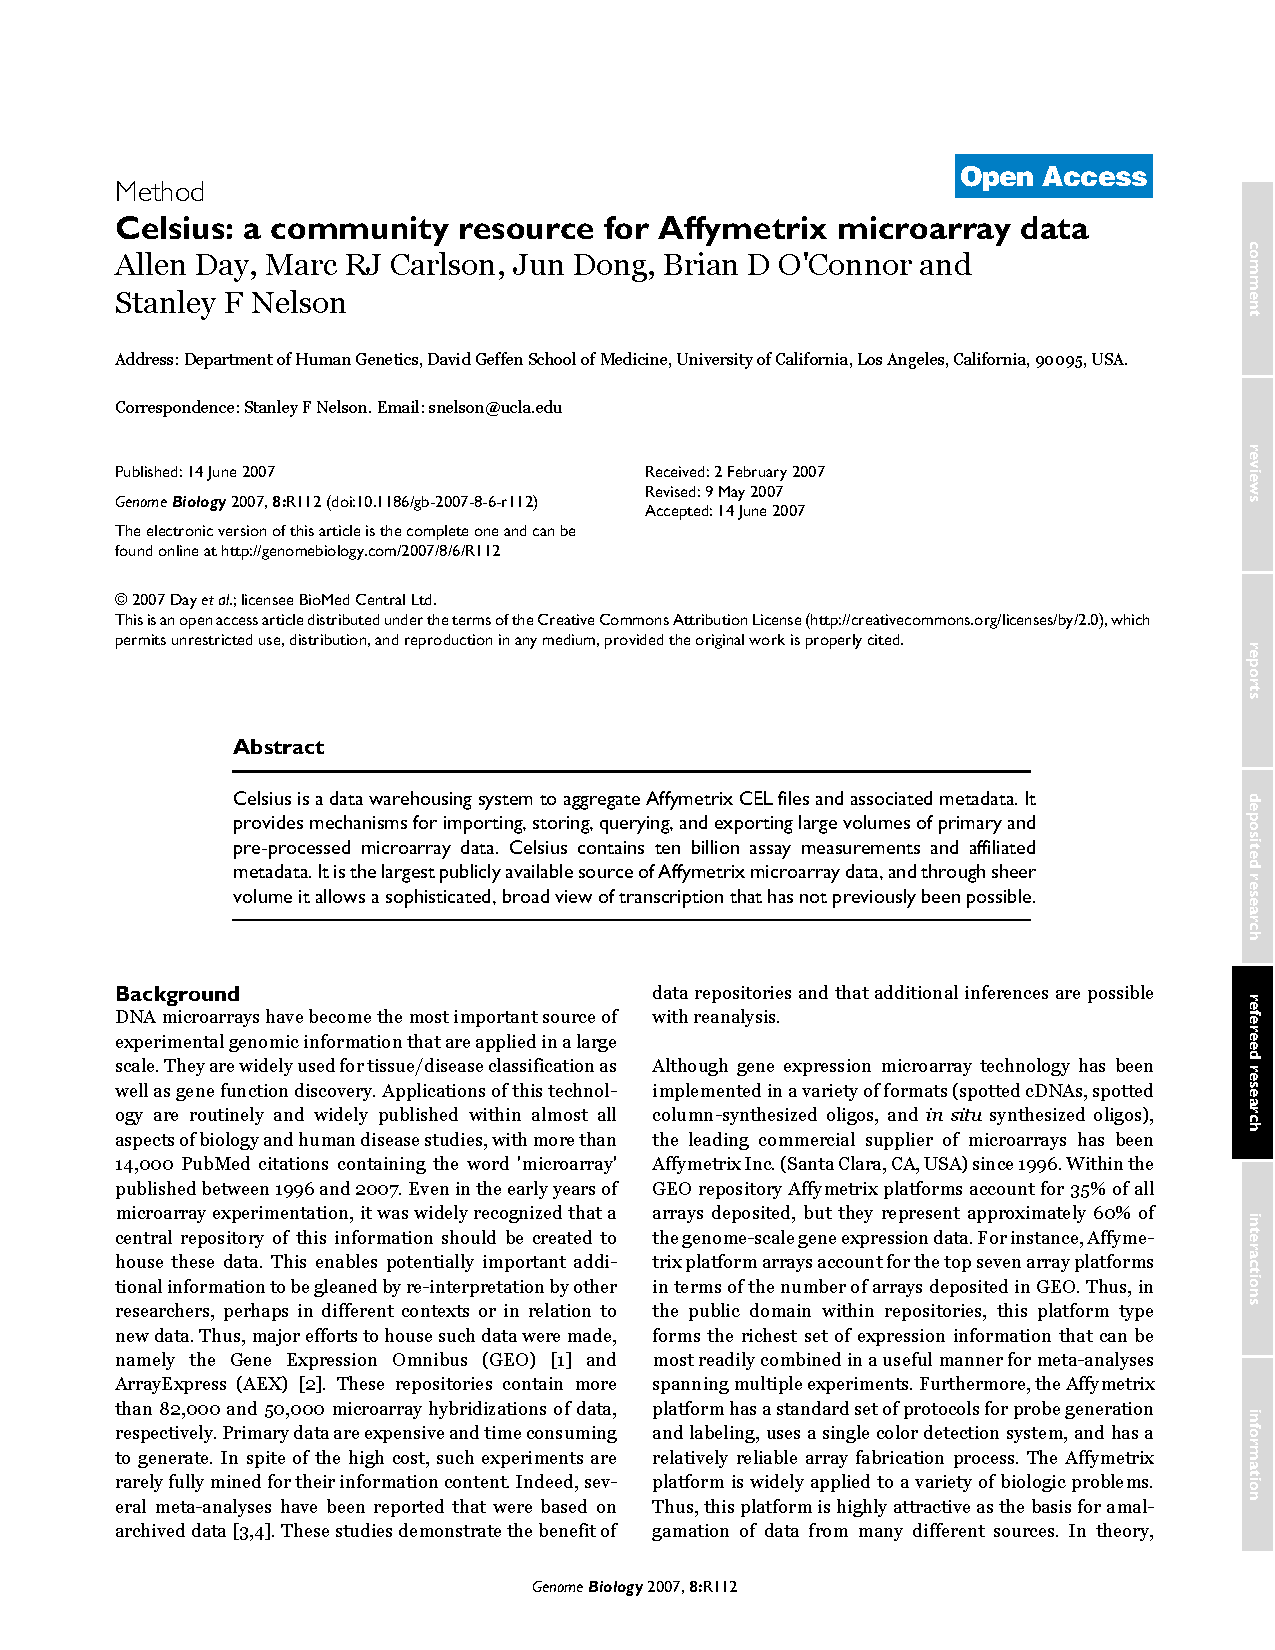
\includepdf[pages=1-13, scale=.75,
            trim=5mm 15mm 10mm 25mm,
            clip, pagecommand={}]{publications/celsius.pdf}

%\chapter{Scalable Classification of Affyemtrix Microarray Samples}
%There are many difficulties facing the researcher who wishes to have a
high-level view of the ``state-space'' of the human transcriptome, or the
complete set of stable states allowable by the transcriptional regulatory
network of the human genome \cite{XXX}.

The first of these difficulties is the assembly of measurements of gene
transcription across as many phenotypic conditions as possible.  The second
difficulty is pre-processing those measurements so that they may be used
together in a single meta-analysis.  A solution to the problem of
pre-processing was presented by XXX, et al \cite{genelogic}, and an
implementation of that method was incorporated into Celsius, a microarray
database warehouse system previously published by these authors \cite{celsius}.
The scope of Celsius was to identify, amalgamate, and preprocess all publicly
available Affymetrix microarray data.  While such a data set is interesting for
investigations of low-level studies of microarray behavior, it is not by itself
particularly useful for understanding the structure of transcriptome state
space.  The problem is not that the state space cannot be observed, but rather
that it is lacking labels.  What is needed is a mapping between anotomical,
physiological, and cellular structures phenotypes and regions of the space.

We present here our construction of an automated system that is able to assign
labels to some of the space described.  We demonstrate the usage of flat
(random forest) and hierarchical (pachinko machine) classification algorithms
to assign high-level phenotypic labels to many samples in the Celsius data
warehouse.


%#####
PMID_17453049	Revealing static and dynamic modular architecture of the eukaryotic protein interaction network.
PMID_18007649	The road to modularity.
PMID_17353930	Network-based prediction of protein function.

%
%\includepdf[pages=2-13, scale=.75,
%            trim=5mm 15mm 10mm 20mm,
%            clip, pagecommand={}]{publications/celsius.pdf}
%
% biopackages manuscript - margins ok
\chapter{Biopackages.net: Bioinformatics Libraries, Applications, and Data as Operating System Packages}
% \title{Biopackages.net: Bioinformatics Libraries, Applications, and Data as Operating System Packages}
% \author{
% Allen Day\correspondingauthor$^{1,2,\ddag}$ \email{Allen Day\correspondingauthor - allenday@ucla.edu} \and
% Brian D. O'Connor$^{2,3,\ddag}$ \email{Brian D. O'Connor - boconnor@ucla.edu} \and
% Jordan Mendler$^{1}$ \email{Jordan Mendler - jmendler@ucla.edu} \and
% Jared Fox$^{1,4}$ \email{Jared Fox - jaredfox@ucla.edu} \and
% Stanley F. Nelson$^{1}$ \email{Stanley F. Nelson - snelson@ucla.edu} \and
% Lincoln D. Stein\correspondingauthor$^{2}$  \email{Lincoln D. Stein\correspondingauthor - lstein@cshl.edu}
% }

%\maketitle


%%%%%%%%%%%%%%%%%%%%%% ABSTRACT
%\begin{abstract}

\section{Abstract}

\paragraph*{Background:}
As biological science becomes more quantitative, it is increasingly dependent on large and
complex computational infrastructure.  Large-scale systems exist upon which 
analyses can be done, but efforts are often foiled by the analytical software itself,
which is frequently of pre-production quality, poorly documented, and difficult to locate, install and configure.

\paragraph*{Results:}
We have created Biopackages.net: a repository of libraries, applications, and data sets
that are commonly used in computational biology. This resource solves the problem of software installation by providing pre-configured packages for many of the data and software most commonly used in the biological sciences.  We have also created a ``build farm''
-- a software application that allows software packages in the repository to be automatically adapted to
new operating systems and hardware architectures.

\paragraph*{Conclusions:}
Using software available from the Biopackages.net repository in conjunction with a
mature cluster management product lowers the barrier to entry for addressing
large-scale problems in computational biology and bioinformatics.  It streamlines the initial setup and maintenance of complex software collections allowing scientists to focus more time on research and less time on configuration.  More information is available at \url{http://biopackages.net}.

%\end{abstract}

%%%%%%%%%%%%%%%%%%%%%% INTRODUCTION
\section{Introduction}

As biological science becomes more quantitative, it is increasingly dependent
on large and complex computational infrastructures.  Scalable and modular clustered
computer systems are now essential for analysis and hypothesis generation from
current high-throughput assay technologies.  While advances in the scientific computing
community have led to the creation of systems that use clustered computer systems to
increase productivity, e.g. the Rocks environment \cite{rocks}. These efforts seldom address another part of the
problem, namely \textit{deploying} research-grade software on these systems.  This latter problem is not trivial, and the associated
productivity loss is a major obstacle in the advancement of computational life science.

The degree to which software increases productivity can generally be evaluated
along three axes: utility, accessibility, and usability \cite{keates}.  Applications and software libraries produced in life science research environments
are of great utility.  They provide means to represent, store, retrieve, and manipulate
biological data.  However, even the best of these applications and libraries typically have low marks
for accessibility and usability.

Research code is often not readily accessible because it is of prototype
quality, with poorly documented interface, installation and configuration
mechanisms, and comes with no formal support or guarantee that it will compile,
execute, or be otherwise usable on the platforms and operating system combinations of end users.  Usability suffers from poor documentation, as well
as from inconsistent and often rough-cut user interfaces.  Ease of use has also been
lacking in the research code environment. Software installation has historically
been a painful process that involves README files, configuration settings, and
other processes requiring active human interaction.  This condition frequently
persists even within popular and widely used scientific software, likely due to a
deficiency in knowledge of and adherence to software ``best practices'' as
previously posited \cite{baxter}.

%XXX
The primary aim of the Biopackages.net project is to increase the productivity
of life science informatics environments through software packaging.  By
compiling, testing, and configuring software, we are able to greatly increase the
accessibility and usability of it.  Another benefit of packaging is that it is possible to
compile and configure complementary packages to be aware of and interact with
one another and the underlying OS.  This creates an environment
with greater utility than the sum of its parts.

%Considering the extra problems introduced by significant increases
%in scale, as in the case of administering large numbers of systems that all
%need to have similar utilities installed -- this stratified
%installation procedure simply does not scale \cite{couch}.  One of the
%strategies used to combat these stratified installations is the use of thin
%clients. Thin clients are machines on a network that retrieve data and programs
%from central repositories on the network and typically contain no local
%customizations. This technique allows system administrators to update all of
%the clients by making a software change on the single central repository.  One
%drawback to this method is that the central repository quickly becomes very
%complex, since each user will likely have special applications or
%customizations that they need to use. In this scenario, users who install
%software onto the central repository can frequently corrupt the installations
%of other users' applications \cite{couch}. This requires the system
%administrator to spend a great deal of time installing, upgrading, and
%troubleshooting software installations.  We are not convinced that the thin
%client approach is practical, in that rather than truly factoring out the
%administrative overhead, it has instead shifted the problem into a mode of
%repository maintenance.  Thin clients also have a performance price in life
%sciences applications that are frequently I/O bound and are better served by
%local storage media than media available through the local area network.

%%%%%%%%%%%%%%%%%%%%%% RESULTS
\section{Results}

The Biopackages.net software repository is available at
\url{http://www.biopackages.net/}.  At the time of writing more than 3800 software packages %XXX 3800
are available for several versions of the Fedora Core and CentOS Linux operating systems on
i386 and x86\_64 architectures, as well as a shared set of
architecture-independent (noarch) packages.  All packages currently provided
are prepared using the Biopackages.net build farm which in turn employs the RPM
Package Manager \cite{herrold}, a suite of utilities for installing and
maintaining software on a computer system.

\subsection{Provided Applications and Libraries}

Biopackages.net aims to provide a software repository as broad as possible
within the discipline of open-source bioinformatics.  Research interests of the
contributing authors that are outside the scope of this manuscript include
complex disease gene mapping and gene expression analysis.  As such, there is a
trend for the content of the repository to reflect these topic areas.  Even so,
we have attempted to include many of the commonly used bioinformatics data
sets, libraries, and applications.  Data sets provided include: ontologies
provided by the National Center for Biomedical Ontology, standard Affymetrix
GeneChip data sets, and recent genome assemblies for several commonly studied
organisms pre-formatted for use with the sequence analysis programs BLAST,
ePCR, and BLAT \cite{ncbo,blast,epcr,blat}.  For libraries, the
popular Bioconductor and Bioperl \cite{bioconductor,bioperl} libraries are
available, as well as the NCBI Toolkit libraries supporting the BLAST
application already mentioned.  Other applications available include the
Generic Genome Browser, the BLAT server, Textpresso, EMBOSS, and Turnkey/GMODWeb
\cite{gbrowse,blat,textpresso,emboss,gmodweb}.

\subsection{Using the Biopackages.net repository}

Software provided by the Biopackages.net servers can be browsed and downloaded
directly using a web browser, then installed on the target system with the
\texttt{rpm} command-line utility.  Using the RPM Package Manager
reduces the amount of human interaction to two steps in most cases: users can
simply retrieve the RPM file and then install with a single command.  In
addition to ease of installation, RPM also provides a wide array of features
that make it superior to many other software packaging formats \cite{hess}.

While this method of installing software is possible we also support -- and
recommend -- using automated software utilities for package dependency
resolution and installation, such the Yellow dog Update Manager (Modified), or
\texttt{yum} \cite{vidal}.  \texttt{yum} allows users to install desired packages in an automated
fashion with a single command.  The Biopackages.net website provides
instructions and a single RPM that can be downloaded and installed to make the
user's installed version of \texttt{yum} configured to be aware of how to obtain and install packages from the Biopackages.net repository.  \texttt{yum} is well
suited for bioinformatics research because many of our applications and
libraries are considered high-level from the point of view of the
OS and have a deep and broad graph of software dependencies.  For example,
consider the partial software dependency graph shown in Figure
~\ref{fig:bp_depgraph}.  Installation of the \texttt{das2-server} package
requires the \texttt{chado-Hsa} package, which in turn requires two other
packages to be installed, and so on.  Installation of these high-level packages
frequently requires the manual retrieval and installation of possibly hundreds
of other packages in the dependency graph \cite{bodnar}.

%\subsection*{Performance}

%Many aspects of system performance, such as network I/O and disk usage can be
%affected by using Biopackages.net repository, with the gains or losses
%incurred through use of this repository depending on the machine and network
%configuration at a particular site.  As this is the case, we have chosen to
%evaluate performance gains of using the Biopackages.net repository in terms of
%human administrative costs, which should be consistent between sites.
%\textbf{Bar chart of build+install vs install time here}

\subsection{Build Farm}

Software packages for the biopackages project are built using a software system
spread across multiple machines.  In the system a single machine acts as the
master control node (MCN) and orchastrates the process of building a given
package.  Individual machines act as build nodes where a package and its
dependencies are built.  The build farm's MCN manages the building of packages
and their dependencies by assigning the jobs to particular build nodes.  On
each build node the resolve\_deps.pl script manages the process of recursively
building a given package and all its dependencies.  This "build farm" allows
the same package to be built on multiple operating systems and architectures in
a parallel fashion.  This flexible framework allows new platforms and operating
systems to easily be added.  This build farm approach is flexible and requires
little human interaction to build all packages for a particular platform and
operating system. In this way, biopackages is more than just a collection of
software and data packages.  It provides a complete framework for adding and
building new software packages across a variety of platforms and operating
systems with minimal effort.

%%%%%%%%%%%%%%%%%%%%%% DISCUSSION
\section{Discussion}

The Biopackages.net repository is a large collection of software developed that
is relevant to -- and in many cases specifically developed for -- information
management and computational analysis in the biological sciences.  Software is
packaged using the RPM Package Manager and distributed using the Yellow dog
Updater (Modified), both of which are commonly used software management
utilities for Linux-based computers.  At the time of this writing the
repository contains more than 3800 packages  for Fedora Core Linux, Centos %XXX 3800
Linux, and Apple's OS X Darwin 10.4.

A large fraction of the package growth rate can be accounted for by (a) the
recompilation of packages for all platforms, and (b) minor adjustments to
package contents and metadata, analagous to debugging and documentation in the
software development process.  While this type of growth is necessary for the
Biopackages.net repository to remain usable on a variety of platforms, it is
less interesting and less desireable than repository growth to include new
software from the research community, as well as new versions of existing
software.

Substantial effort must be invested to maintain the repository in a useful and
up-to-date state, but it is an overall win for the bioinformatics community if
users buy in to the system, as it allows bioinformatics-specific system
updates to be treated as a service, effectively factored out by delegation to a
group of specialists \cite{nation,soap}.  The amount of effort necessary
to identify and incorporate new software from the community may also be
partially mitigated if users of the Biopackages.net repository reaches a
critical mass.  In this scenario, authors of software are able to attain more
prominence and citation rank by ensuring their software is readily available to
the largest number of users.

\subsection{Licensing}

Academic software is commonly available through a dual-licensing model in which
academic or not-for-profit research use is freely granted, but enterprise-class
users are required to pay for use.  The licensing terms are typically
prominently displayed on the authors' software download pages, and are
difficult to miss.  One potentially adverse effect of using the Biopackages.net
repository through \texttt{yum} is that hundreds of license terms can be
implicitly agreed to with only a few keystrokes.  While this is typically not a
problem for academic users, it may create legal difficulties for users in the
enterprise.  We encourage all users to closely examine all pacakge metadata to
ensure they are entitled to use the software under the terms in which it is
distributed via the Biopackages.net repository.  One possible mechanism to ease
the burden on end users is to partition the repository's software based on
license permissiveness, and is a future goal of the
Biopackages.net project.  Future goals also include contributing to larger and
more general-purpose repositories, such as \url{http://pbone.net/} and
\url{http://atrpms.net}.

\subsection{Non-RPM Systems}

We are also interested in extending the scope of the project beyond operating
systems that use the RPM Package Manager natively.  In our preliminary work in
this area, we focused on Apple MacOS X 10.4 and Cygwin for Microsoft Windows
XP, and used the RPM and \texttt{yum} ports available on these systems.  While it was
possible to use RPM and \texttt{yum} to manage installed software on these systems, it
was neither trivial nor elegant.  The essence of the problem lies in the fact
that at their lower levels, software dependency graphs rely on basic software,
such as the Bourne shell, or the Apache HTTP server.  These basic packages are
available and usable by RPM-installed software on non-RPM-native systems, but
the RPM-based utilities cannot verify dependency integrity.  Our solution to
this problem is to provide virtual packages that claim to provide software
(such as Apache), but actually do nothing and defer to the base system packages
to provide the functionality.

There is also potential to convert Biopackages RPMs into non-RPM formats for
use on a wide breadth of UNIX types. While RPM support has been ported to most
versions of UNIX and Linux, many of these OSes were initially
developed with other binaries in mind. Distributions based on Debian Linux,
for instance, are native to deb packages while Sun's Solaris and many other
UNIXes are native to pkg. Slackware Linux uses .tgz packages, while
Stampede Linux uses .slp packages. Fortunately for maintainers tools has
been developed to convert packages between these many formats. One such
software is Alien which allows conversion between the above named package
types. This creates the prospect of developing Biopackages branches for
different package formats to attract users for whom RPM is not a viable option.

%%%%%%%%%%%%%%%%%%%%%% METHODS
\section{Methods}

\subsection{Package Creation}

The first step in creating a software package is to obtain the package's source
material, or sources, from an upstream provider.  For a software library, this
may be a tarball of C++ files, and for a genomic data set may be several FastA
files.

The second \textit{optional} step is to create patches that modify the package
sources to be compatible with the target platform for installation.
Modifications typically do not change the core functionality of the software,
but customize the software or software installer slightly to be compatible with
the target platform or related software libraries and applications.

The third step is the creation of a metadata file, which for RPM based systems
is called a spec file.  The spec file references the source and patch
files and includes instructions for performing the configuration and
installation of the software.  Additionally, the spec file lists all other
packages that are required in the build- and
install-phase.  The packages depended upon may differ for build and install phases, and may also be conditional by platform .  The spec file also contains other package-related metadata, such as license details and
type of package (library, database, application, etc).

\subsection{Package Version Control and Platform Targeting}

After being initially written, the spec file is then converted to a spec.in
file and imported into the Biopackages.net Concurrent Versions System (CVS)
repository.  The Biopackages.net project abstracts the spec file metadata one
step further for two reasons.

First, the spec file contains a revision metadata field for package version
information, but provides no mechanism for automatic managment of version
numbers.  Likewise, it contains a changelog metadata section for describing
how a package has evolved over time, but does not provide a utility for
tracking changes.  CVS does both automatic revision and changelog tracking, but
in a different format than is required by RPM.  A simple search-and-replace
preprocessing step is sufficient to map the CVS sections for versioning and
changelogs (\texttt{\$Id\$} and \texttt{\$Log\$}) to the corresponding RPM spec
file sections (\texttt{\%revision} and \texttt{\%changelog}).  The
Biopackages.net build system includes a utility to perform this task.

Second, spec file syntax does not allow all portions of the file to be
conditional based on aspects of the platform. With the use of a single spec
file for multiple platforms, it is important to optionally specify different
build and installation requirements for the same package on different Linux
distributions. This is because of the variation of libraries included with a
given package across distributions. As an example, a default Perl on Fedora
Core 2, may include a Perl library that is not included in the default Perl
installation of Fedora Core 5. Therefore it is important to specify this
library as an additional requirement for Fedora Core 5, while unnecessary for
Fedora Core 2. RPM is limited in its ability to include conditional statements
in the build and installation requirments sections of the spec file. Therefore
the solution we have implemented is the inclusion of a platform specific
\texttt{if} control structure in the spec.in file.  This is translated from a
conditional statement to the resulting package dependency when the spec.in file
is converted to a spec file.

\subsection{Package Compilation}

Package compilations are performed on a self-contained Build farm that
contains all of the OS distributions we target. Using VMWare virtualization on a
64-bit AMD based machine, we are able to simultaneously run multiple
32- and 64-bit x86 architecture virtual machine (VM) instances, each with a
different OS and virtual architecture.  This allows us to build packages for
many different platforms simultaneously.

The RPM construction process uses the Sun Grid Engine (SGE) cluster management utility to
orchestrate construction of a given \textit{target} package for multiple platforms, and is illustrated in ~\ref{fig:bp_buildfarm}.
This process is initiated by iterating over all platforms targeted for construction, and interacting with the
SGE Master Control Node (MCN) to build those packages.  MCN manages all VMs and ensures
that each request to build \textit{target} for a particular platform is delegated to the correct VM.  Once
delegated to a VM, package construction process can be divided into three phases:
staging, building, and cleanup.  These are illustrated in Figure \ref{fig:In2rpm}.

In the staging phase, \textit{target}'s metadata is converted from the CVS \texttt{RCS} to \texttt{rpmbuild}
format, and all packages that are required to build \textit{target} are identified and installed.  This
process is coordinated by the \texttt{resolve\_deps.pl} script.  It begins by parsing \textit{target}'s
metadata to identify all packages that are depended upon for build or install of \textit{target}.  Each of
these depencies in turn has its dependencies identified, and so on, recursively.  When the terminal
packages of the dependency graph are reached, the recursive process traverses back toward
\textit{target}, and at each step installs the dependency to ensure that all requirements in the graph
have been installed.

In the building phase, \textit{target}'s metadata is used to construct the RPM package.  This is
done with the \texttt{rpmbuild} utility, which typically invokes several other scripting tools and
software compilers to prepare the \textit{target} software for the VM's platform.

Finally, cleanup phase takes place.  All packages that were installed to satisfy the dependency are
uninstalled.  This restores the build system to a ``clean'' state ready for the next scheduled build.
The rpm file for \textit{target} is archived to a repository where all complete packages are moved to shared storage and
made available to the public via a web server.  Log files created during the staging and build phases
are also archived to shared storage for post-processing.  Examples of post processing include the generation of build
reports, identifying VM-specific problems, and detection and re-queueing of failed builds.

After all packages have been iterated over and all requests scheduled with the MCN have completed,
the packages in the RPM repository are indexed using the \texttt{createrepo} command.  This enables
\texttt{yum} clients to connect to the web server and install packages.

\subsection{Package Deployment}

Built RPMs are automatically written to a shared NFS volume that is
accessed by the Biopackages web server. Packages are initially placed into a
``testing'' repository corresponding to distribution and architecture. After
enough testing of package stability, RPMs are migrated to the ``stable''
repository. On the web server, a nightly cron job automates the creation of
\texttt{yum} and \texttt{apt} headers for all platforms of both the stable and testing
biopackages repositories. From this server, packages are served over HTTP and
NFS to both local and external clients that make requests.

\subsection{Package Installation}

Once headers are generated on the web server, the user has the choice of
several installation methods for a given RPM. The native Red Hat method is to
use RPM to perform the installation directly from the web server, or from a
local disk the package has been downloaded to. While this allows automated
downloading and installation of a package, RPM is limited in its inability to
perform dependency resolution and therefore requires manual installation of
dependencies. Therefore an easier installation method is through the use of \texttt{yum}
or \texttt{apt}. \texttt{yum} allows for easy installation from a software repository by locating
and downloading the desired packages and all of its dependencies in one
automated transaction. \texttt{apt} serves a similar purpose as \texttt{yum}, originally being
ported from Debian Linux for use with RPMs. Therefore some users are more
comfortably with and prefer the syntax and capabilities of \texttt{apt}.

Another decision to be made by the user is if they would like to use ``testing''
RPMs. \texttt{yum} and \texttt{apt} make it possible for a user to specify which repositories
they prefer, and which repositories are only to be used with manual input. This
allows a user to disable regular use of the ``testing'' repository, while allowing
manual overriding when a package is present only in the ``testing'' repository.

\subsection{Package Quality Assurance}

In maintaining a software repository, a crucial issue is adopting a method of
ensuring stability and quality of packages and identifying problematic
software. A two tiered repository approach helps separate production tested
packages from more newly built RPMs. Newly built RPMs are placed into the
Testing repository, where they are served to both local and external users for
functional testing to be performed. This allows assurance of proper
documentation, configuration files, log files, runtime scripts and other
software functionality before a package is deemed ``production ready'' and
migrated to the ``stable'' repository. It is in this testing period that bugs are ideally
discovered and reported by users and developers, to allow fixes to be made
before the package is moved to the ``stable'' repository. Most Testing packages are
considered to be mostly stable and are immediately implemented on local compute
nodes, however a separate Stable branch adds an extra level of quality control
for production environments.

\section{Figure Captions}

\subsection{Figure 7.1}

Packages are represented by
boxes, with grey provided by the OS distribution, and white provided by
Biopackages.net.  Packages may rely on other packages, either at build- or
install-time.  Solid head dashed lines indicate a n installation dependency,
hollow head dashed lines indicate a build dependency, solid head solid lines
indicate both an installation and build dependency.

\subsection{Figure 7.2}

A spec.in file is preprocessed to form
a spec file, which is processed by the \texttt{rpmbuild} utility along with the
package source files to form architecture-specific packages and a source
package that contains the .spec file and source files.

\subsection{Figure 7.3}

A controlling script
observes the state of the package repository, and spawns jobs to build missing
packages via a master/slave cluster managmement system.  Packages are build and
uploaded to a shared filesystem, where they are then made available over the
network to clients wishing to install software.


% %%%%%%%%%%%%%%%%%%%%%% ACKNOWLEDGEMENTS
% \section{Acknowledgements}
% 
% We acknoledge the following individuals for their help in the development,
% documentation, testing and maintenance of the software and systems described
% here: Patrick Alger, Andrew Helsley, and Victor Ruotti.  Additionally, we thank
% Scott Cain, Steve Chervitz, and Todd Harris for discussion related to the
% design of the project architecture.  We thank Ling Lee for designing the
% Biopackages.net website.  This work was supported by NIH grants XXXXXXXXXXXXX.

%%%%%%%%%%%%%%%%%%%%%% FIGURES
\pagebreak
%\section{Figures}

\begin{figure}[p]
\includegraphics[width=12cm]{figures/Bp_depgraph.png}
\caption{Partial package dependency graph.}
\label{fig:bp_depgraph}
\end{figure}

\begin{figure}[p]
\includegraphics[width=12cm]{figures/In2rpm.png}
\caption{Package compilation process.}
\label{fig:In2rpm}
\end{figure}

\begin{figure}[p]
\includegraphics[width=12cm]{figures/Bp_buildfarm.png}
\caption{Biopackages.net build farm architecture.}
\label{fig:bp_buildfarm}
\end{figure}


%%%%%%%%%%%%%%%%%%%%%% REFERENCES
\pagebreak
\bibliographystyle{plain}
\bibliography{biopackages_3-16-07}




% gmodweb manuscript - margins ok
\chapter{GMODWeb: A Web Framework for the Generic Model Organisms Database}
%$Id: gmod_web_03-25-07.tex,v 1.1 2007/04/04 22:06:26 boconnor Exp $

% Abstract

\section{Abstract}

% No more than 250 words, with second para for web address.  \cite{gbrowse}

The GMODWeb project is a software framework designed to speed the development
of websites for Model Organism Databases (MODs).  GMODWeb is part of the larger
Generic Model Organisms Database (GMOD) initiative which provides
species-agnostic software tools and data models for representing curated model
organism system data.  Users of GMODWeb can browse and search through many
different data types including genomic features and annotations, stocks,
literature references, and genomic maps. It is also integrated with other GMOD
tools such as GBrowse, AmiGO, and Textpresso. To assist development of new MOD
sites end-to-end examples of fully customized and integrated GMODWeb instances
for the \emph{H.  sapiens} and \emph{S.  cerevisiae} genomes have been created.
The recently inaugurated ParameciumDB also uses GMODWeb as its core website
technology for presenting key data of interest to this MOD community.  GMODWeb
is built on the flexible Turnkey web framework and is freely available under an
open source license from \url{http://turnkey.sourceforge.net}.  User
documentation, support forums, and source downloads are available at this site
while pre-packaged versions for Linux distributions are downloadable at the
Biopackages repository for bioinformatics software
(\url{http://biopackages.net}).


% Introduction

\section{Introduction}

Model Organism Databases (MODs) are built around the information needs of
scientists working on a single model organism or group of closely related
organisms.  Examples of MODs include Flybase (\url{http://www.flybase.org})
\cite{PMID_16381917}, Wormbase (\url{http://www.wormbase.org}) \cite{wormbase}, the
Mouse Genome Informatics (MGI) Database (\url{http://www.informatics.jax.org})
\cite{mgid}, the \emph{Saccharomyces} Genome Database (SGD)
(\url{http://www.yeastgenome.org}) \cite{sgd}, Gramene
(\url{http://www.gramene.org}),  a monocot genomics database
\cite{PMID_16381966}, and ParameciumDB (\url{http://paramecium.cgm.cnrs-gif.fr})
\cite{ParameciumDB}.  MODs provide scientists with access to information about
genomic structure, phenotypes, and mutations along with large-scale datasets
such as those generated by gene microarray experiments, SNP analyses, or
protein-protein interaction studies.  A key concern for any MOD is to provide
well-designed and convenient community tools for accessing this information.
All MODs create websites to fulfill these needs, an expensive and
time-consuming prospect. As many more model organisms are sequenced the costs,
in terms of both time and funds, of independently developing schemata and
web-based tools will become prohibitive.

Recognizing this duplication of work, the NIH and the USDA Agricultural
Research Service funded the Generic Model Organisms Database (GMOD) project
with the goal of developing flexible applications that can be used across all MODs.
The result is a collection of database and web tools that can be mixed
and matched to meet the requirements of new MODs.
%These tools address needs for representing and visualizing both genetic and
%physical maps, storing and searching literature curations, and browsing
%ontological annotations, along with an extensible architecture for a MOD
%website development.
To date, this effort has produced several high-profile components. A generic
and modular relational database schema, called Chado, provides the core
mechanism to store genomic features, information on gene function, genomic
diversity data, literature references, and other common data types.  Other
popular GMOD tools include Apollo \cite{apollo}, an application for genomic
curation, GBrowse \cite{gbrowse}, a web-based genomic browser that can
effectively display genomic features across megabases of sequence, and
Textpresso \cite{textpresso}, a web tool for literature archiving and
searching. While several solutions exist for representing genome annotation
data on the web, such as Ensembl \cite{ensembl} and the UCSC genome browser
\cite{PMID_12045153}, no solution exists for representing the full variety of
data types needed for a MOD.  In this paper we describe GMODWeb, a flexible and
extensible framework for creating a MOD website that integrates with other GMOD
tools and accommodates all the data types needed for a model organism database.

% NOTE: Lincoln removed this from Draft3
%Every MOD needs a web presence to disseminate information about the model
%organism.  Other web frameworks for presenting biological data exist, such as
%GenBank \cite{genbank} and Ensembl \cite{ensembl}, but their focus differs
%from what is needed for a MOD.  While GenBank focuses on genomic feature
%archiving and Ensemble on whole genome annotations, a MOD website need to
%present annotations and data for just one organism and present it in a way
%that is helpful for the MOD community as a whole.  The emphasis for these
%species-specific sites is more centrally placed on genome annotation and the
%web interfaces to these MODs need to primarily share these annotations with
%end users. The GMODWeb application has been designed closely around the common
%GMOD Chado schema.  Since the schema forms the basis for all the MODs, a web
%tool that accurately represents the schema and allows an end user to browse
%the information contained within is key.  GMODWeb has been specifically
%created to allow end users to explore the features and annotations stored in a
%Chado database and to link out to other websites and tools including
%BlastGraphic \cite{blast} \cite{blastgraphic}, Textpresso \cite{textpresso},
%GBrowse \cite{gbrowse}, among others.  To date, two GMODWeb example sites have
%been created, for human and yeast.  These are available as part of a sample
%GMODWeb install and will help future MODs by providing concrete examples of a
%GMODWeb setup that can be directly adapted and reconfigured for other model
%organism databases.  Already, ParameciumDB \cite{parameciumdb}
%(\url{http://paramecium.cgm.cnrs-gif.fr) has used these examples to create a
%GMODWeb instance.


\section{Results}

\subsection{GMODWeb Architecture}

GMODWeb is based on the Turnkey (\url{http://turnkey.sourceforge.net}) site
generation and rendering framework which consists of two distinct components.
The first is a code creation tool (Turnkey::Generate) that produces a Model
View Controller (MVC) based website given a database schema file \cite{mvc}. In
the case of GMODWeb this is the Chado schema.  The second Turnkey component
(Turnkey::Render) is a page-rendering module that links the generated MVC code
to an Apache webserver (\url{http://apache.org}). This portion of the Turnkey
framework uses a collection of open source perl modules and the popular
mod\_perl webserver plugin (\url{http://perl.apache.org}). Each Turnkey
component is used in a different phase of website construction.  While the
MVC generator automates the creation of most site code, the page-rendering
module handles the response to user requests received by the webserver.

Turnkey, and GMODWeb by extension, is strictly divided into MVC layers.  This
style of abstraction is a useful tool for organizing a web application into
manageable layers and improves the overall organization of the software.
Likewise, the active code generation approach used by Turnkey, which is similar
to the Object Management Group's (\url{http://www.omg.org/mda}) Model Driven
Architecture (MDA) proposal, is especially useful for the GMODWeb project
because underlying changes in the data model are quickly and easily integrated
into the application \cite{mda}.  For example, the inclusion of new database
modules in Chado can be easily accommodated by regenerated the Turnkey site
from the database schema file. GMODWeb is produced by simply applying
customizations, a GMODWeb "skin", to the Turnkey website auto-generated using
the Chado schema. This decoupling of user interface customization from
underlying data structure makes the GMODWeb application easy to extend,
customize, and maintain. Figure 1 shows the close relationship between GMODWeb
and Turnkey.

%FIXME: there's a lot more that can be added here with more talk about MDA and
%MVC being top on the list.  

\subsection{GMODWeb Site Generation and Rendering}

The creation of a Turnkey site, such as GMODWeb, beings with a SQL schema file
used to define the tables in a database and how they relate to each other.
This file is abstracted into relationships between objects forming a Directed
Graph (DG).  Turnkey::Generate uses the perl module SQL::Translator to perform
this conversion from a SQL schema file to a DG object model
(\url{http://sqlfairy.sourceforge.net}).  For example, in the Chado schema a
{\texttt feature} table stores information about genomic features such as mRNAs or
genes.  This table is linked to many other tables, such as the {\texttt synonym}
table via the {\texttt feature\_synonym} table.  The Turnkey::Generate script
creates objects representing each table ({\texttt feature}, {\texttt synonym} and {\texttt
feature\_synonym}) and their individual data fields.  It then creates links
between these objects to mimic the relationships encoded by the schema, in this
case linking the {\texttt feature} and {\texttt synonym} tables.

Using the relationships encoded by the DG, Turnkey::Generate produces an MVC
mod\_perl website.  
%An MVC-based application is desirable because it segments an application into
%components that communicate with a datasource, others that render the user
%interface, and controller components that manage the flow of information.
%This style of programming is commonly used for web development and the
%division into these application layers provides abstraction and flexibility.
Each layer of the MVC framework is created using Template::Toolkit templates.
The model layer, which handles the flow of information to and from the
underlying database, is created using a template to produce Class::DBI-based
objects (\url{http://wiki.class-dbi.com}).  Class::DBI is a convenient tool to
connect and retrieve information from the database because it abstracts complex
SQL queries into easy-to-use object calls.  Controller objects, called atoms in
the Turnkey framework, wrap the model objects and provide an abstraction
between the view and model objects.  They also include the logic necessary to
bring these two layers together.  The view layer is, itself, implemented in
Template::Toolkit and uses HTML with embedded tags to extract information from
controller objects for display to the end user.  Turnkey::Generate also creates
the Turnkey.xml controller document that describes how model and view objects
are to be combined by the atom controller objects. Figure 2a illustrates the
MVC-based architecture created with the Turnkey::Generate software.

Once created, the output of Turnkey::Generate is configured to work in an
Apache server using the mod\_perl framework.  The process of rendering a page
is handled by Turnkey::Render. When a user requests a certain URL, the
Turnkey.xml document is examined by Turnkey::Render and the appropriate
Class::DBI model and controller atom objects are instantiated. For example, the
{\texttt feature} table described previously has an entry in this XML linking it to
the {\texttt synonym} table through the {\texttt feature\_synonym} table.  This
provides Turnkey::Render with enough information to create atom and model
objects for both the feature and synonym tables.  Following this, the
appropriate template view objects are created and Turnkey::Render uses the atom
controller objects to manage the handoff of objects and template files to the
Template::Toolkit engine for rendering.  The resulting HTML output is then
returned to the client (Figure 2b).

\subsection{GMODWeb Customization}

Customization is an important feature that all MODs require in their web
interfaces.  To accommodate this, key design features were integrated into the
Turnkey framework affecting both the site generation and page rendering
processes.  These include template customization through overriding and
Cascading Style Sheet-based (CSS) layouts (\url{http://www.w3.org/Style/CSS}).
Template overriding provides the ability for MOD developers to create a
customized look and feel for a given type of information being displayed in a
GMODWeb site. For example, the default feature page in GMODWeb was swapped out
for a custom templates that included a GBrowse panel if the feature had a
genomic location, as is the case for a gene or an mRNA transcript feature.
These custom templates would normally be overwritten in an MDA web framework
but Turnkey allows site designers to create and persist these modifications.
In addition to template customization, layout and styling in a Turnkey site is
accomplished with flexible CSS documents, allowing the MOD developer to
dramatically change the look and feel of the entire site. Not only can colors
and fonts be changed, but element layouts can be reordered.

A combination of these customizations can be grouped together into a "skin"
which can easily be parameterized and switched on the fly.  This makes it
possible for a MOD website to be context dependent and support a "print" view or
completely different color scheme with the same underlying website and
database. For example, a clade-oriented database that provides information on
12 different beetle species could apply a different page color to each species
to avoid user confusion.  GMODWeb was created by taking a Turnkey website
generated from the Chado database schema and applying these types of
customizations to the codebase (Figure 1).   

Demonstration GMODWeb sites have been created for \emph{H. sapiens} and
\emph{S. cerevisiae} and include the basic functionality associated with a
typical MOD's homepage. These sites illustrate the common layout for a Turnkey
website and show the effects of a customized GMODWeb skin. The sample websites
include the ability to search by features and controlled vocabulary (CV) terms
indexed from the underlying Chado database using the open source search engine
Lucene (\url{http://lucene.apache.org}).  Since many data types in Chado are
annotated and linked together through CV terms using various ontologies, such
as the Gene Ontology (GO) \cite{PMID_10802651}, it was important to be able to
query by both data types.  Search results will take an end user to either a
feature or CV term page rendered using customized GMODWeb templates. 

% NOTE: Lincoln removed
%The resulting Turnkey framework is designed to be completely auto-generated yet
%to provide a flexible skin approach to change the look and feel of a site.
%Customized view templates, along with customized CSS and images, can be
%combined to form a skin.  These skins reside in their own directory and are
%persistent when a site is subsequently regenerated.  This allows customized
%interfaces to persist while the underlying database changes.

Browsing a feature reveals several customizations to the default templates.
Figure 3 shows a typical gene feature page using the GMODWeb skin from the
ParameciumDB MOD website.  In this example, the basic layout of a Turnkey page
is evident: the item being rendered, in this case a row from the {\texttt feature}
table, is present as the major content panel while linked tables are
represented as minor panels on the left-hand side.  For this gene feature, two
types of linked data were presented on the left: external references (via the
{\texttt feature\_dbxref} table) and relationships to other features in the
database (via the {\texttt feature\_relationship} table).
%, and results of computational analysis (via the {\texttt featureloc} table).
Customizations of links and panel headings in both the major and minor panels
are shown in this example as well.

% fixme: could add more about link and header cust.

Further customization was used in the major panel to organize information about
the gene feature in an intuitive and helpful way.  Related content, such as GO
term annotations, genomic location, synonyms, and other information, was
included as a summary.  The Turnkey framework's flexibility allows custom
template authors to easily extract this information using the underlying
Class::DBI model objects. In this customized template, simple nested method
calls on the feature model object were used to extract linked information
such as synonyms.  Together these modifications have created a gene page that
can be leveraged across MODs and provide many of the key pieces of information
about genomic features that end users will require. Turnkey pages also contain
an edit link which provides a limited but useful facility for editing record
data.  Authentication is provided by standard HTTP access controls in Apache.

\subsection{GMODWeb Integration}

The example in Figure 3 shows how GMODWeb's templates were directly integrated
with other GMOD projects.  In this page, a GBrowse instance was embedded and
provided not only a graphical view of the genomic neighborhood but also linked
out to nearby genes and other annotations.  In addition to GBrowse, the sample
GMODWeb sites for \emph{H. sapiens} and \emph{S. cerevisiae} include
integration with Textpresso for literature tracking, BlastGraphic for
performing Blast analysis, and AmiGO for controlled vocabulary term
visualization. These dependencies, which are available from the Biopackages
software repository, have been pre-configured to work with the GMODWeb
demonstration sites. Packaging the sample applications and their dependencies
makes installation and configuration a quick and easy task for site developers
and jumpstarts the process of setting up new MOD websites.

In addition to web interfaces, GMODWeb also provides Simple Object Access
Protocol (SOAP) (\url{http://www.w3.org/TR/soap}) bindings for accessing data in an
automated, programmatic way.  This web services approach is designed to allow
savvy end users to interact directly with the underlying GMOD Chado database,
affording bulk access to features contained within the database.  Providing
this tool for GMODWeb's model objects makes data access platform agnostic so
developers can interact with the service using the language of their choice.
Apache2::SOAP (\url{http://search.cpan.org/~rkobes/Apache2-SOAP-0.72}) was used
to bind Class::DBI-based model objects to a SOAP interface.  Unlike XML genome
feature annotation services, such as the Distributed Annotation System (DAS)
\cite{PMID_11667947}, the SOAP bindings present low-level interfaces to
database tables. This SOAP interface is pre-configured and immediately
available for all MOD sites based on GMODWeb.

% FIXME: I need to combine this with the paragraph later on describing SOAP

%The Turnkey-based GMODWeb can be used for more than web-page rendering.
%Because of the flexible nature of the skins approach, and the general utility
%of the Apache environment, two developer-oriented services are available
%through all GMODWeb sites.  First, skins can be created to output XML rather
%than HTML, enabling developers and end users to retrieve information about
%genomic features programmatically.  Second, Apache::SOAP provides automated
%SOAP bindings to the underlying model layer \cite{apache_soap}.  This allows
%savvy developers to directly access a MOD through an easy-to-use and platform
%agnostic web services interface.  These abilities compliment other technologies
%already in use, such as XORT \cite{xort} for producing ChadoXML and DAS
%\cite{PMID_11667947} for producing feature-centric XML documents, and provide
%the means to extend a GMODWeb MOD site beyond simply a web interface. 

\subsection{Case Study: Creating a New MOD Website with GMODWeb and Turnkey}

Paramecium, a unicellular eukaryote that belongs to the ciliate phylum, has
served as a genetic model organism for over half a century and is also widely
used to teach biology. The genome of \emph{Paramecium tetraurelia} was recently
sequenced and annotated at the Genoscope French National Sequencing Center
\cite{ptgenome}. In anticipation of public release of the data from the
sequencing initiative, a project was started in 2005 to develop a Paramecium
community MOD, ParameciumDB. Its immediate objectives were to integrate
the genome sequence and annotations with available genetic data and 
coordinate the manual curation of the gene models by members of the research
community. Ultimately, ParameciumDB should provide a useful resource for the
classroom as well.

GMOD's Chado database schema was well suited for this project because of its
genetic module, which ensured the integration of both the genetic and sequence
data, and its support for describing phenotypes using controlled vocabulary
terms. Another important factor in choosing the GMOD toolkit for ParameciumDB
was the availability of Turnkey and GMODWeb to generate the MOD's website,
since it was anticipated that this would be the most difficult part of the project.

GMODWeb was first tested on a generic installation of Chado, populated with
published data from a previously sequenced and annotated Paramecium chromosome
\cite{Zagulski}.  The next step was modeling the genetic data, which involved
writing a stock sub-module for the Chado genetic module to make it possible to
incorporate data about Paramecium stock collections. Since the Chado database
schema was modified, Turnkey::Generate was used to create a custom website for
ParameciumDB.

The last and most time-consuming step for building ParameciumDB was
customization of the auto generated website layout. The overall design of the
site components (header, footer, feature page, etc) was achieved using
templates and CSS modifications of the GMODWeb skin, resulting in a custom
ParameciumDB skin.  Within the auto-generated view code, the
feature-relationship atom object was modified to make it possible to recover the
complete hierarchy of relationships (e.g.  gene $\rightarrow$ mRNA
$\rightarrow$ exon) from the top-level gene feature, even if the feature page
being rendered concerned a feature type lower in the hierarchy. Additional
static content was added to the site using Microsoft Frontpage including a help
section, project documentation, and announcements
(\url{http://office.microsoft.com/frontpage}).  Finally, commonly used applications
were integrated into the ParameciumDB by linking to other bioinformatics tools,
such as NCBI's BLAST tool \cite{blast}, and to forms for data submission by the
community.

The templates for pages within ParameciumDB were customized using many of the
ideas taken from the GMODWeb sample sites and, in particular, the layout of the
sample gene page.  The elegance of the Turnkey-based MVC site was most apparent
at this level: customization of ParameciumDB was focused on the template view
layer while relatively few changes were required to either the model or
controller objects.  The bulk of the code produced for ParameciumDB was
automatically generated and untouched by the customization process. This freed
developers to work on the effective presentation of MOD data rather than low
level database access or website rendering code.  


\section{Discussion}

Model organism databases (MODs) gather together biologic information on a
variety of important organisms for the scientific community. A key concern for
any MOD is to provide well-designed and easily accessible tools for sharing
this information.  The GMODWeb project was started to provide a simple and
generic solution for quickly creating new MOD websites using the Turnkey
framework.  GMODWeb, by running directly off the flexible and extensible Chado
schema, can accommodate the wide variety of data types and usage patterns that
model organism communities require.  It offers both a clean MVC framework and
pre-built sample websites configured to work with other GMOD tools. Together
these features can greatly streamline the process of new MOD website
development. 

One of the challenges for any framework based on Model Driven Architecture
techniques is balancing auto-generated code tied to a particular underlying
schema with customized layouts for creating compelling and effective user
interfaces.  Turnkey, the technology underling GMODWeb, attempted to solve this
limitation by providing a mechanism for bundling specialized skins with an
auto-generated website.  Since most of the website is automatically created,
designers can focus on the quality of the user interface and not on the
underlying rendering code.  In GMODWeb this translated to extensive
customization of the default feature templates. With the adoption of GMODWeb by
the ParameciumDB project, we anticipate incorporating UI changes and
customization into GMODWeb for the benefit of all future GMODWeb-based MODs.
As additional MODs adopt GMODWeb, we envision the availability of a large
library of site-specific customized templates, which can be adopted, altered
and expanded by subsequent MOD projects.

The rapidity with which ParameciumDB was built, by a very small development
team, is encouraging. For this MOD, data modeling was much more time-consuming
than building the GMODWeb-based website.  In fact, the only difficulty
encountered in implementation of ParameciumDB was not with GMODWeb or Turnkey
\emph{per se}, but with the installation and tuning of mod\_perl and the Apache
web server for use in a production environment. The current availability of
GMODWeb sample sites and installation dependences as pre-compiled software
packages on Biopackages should make this part of a new project much easier for
future MODs. 

% FIXME: this paragraph may be a little repetative with the first
As the model organism database community continues to expand, there will be an
increased need to leverage existing tools to store, query, and present MOD
data.  The GMOD project was created to engineer generic tools to meet these
needs.  GMODWeb was designed to quickly create MOD websites based on the easy
to use, customize, and update Turnkey framework. A GMODWeb MOD site provides
not only the ability to browse and search MOD data but it also forms a key link
to other tools.  As future applications and components become available,
GMODWeb will continue to act as a natural point of integration and a central
hub for the display of MOD data to end users.


\section{Methods}

\subsection{Availability}

Turnkey and GMODWeb are both available as a source code files from Turnkey's
website (\url{http://turnkey.sourceforge.net}) and as pre-compiled packages for
various Linux distributions from the Biopackages repository for bioinformatics
software (\url{http://biopackages.net}).  All dependencies are provided using
the Red Hat Package Manager (RPM) (\url{http://www.rpm.org}) and integration
with other programs, such as GBrowse, is accomplished using this same package
management system.  When a MOD installs GMODWeb via RPMs, a pre-configured
GBrowse, Blast server, Textpresso, and other applications are installed and
configured to work within GMODWeb immediately. Table 1 shows the software
dependencies for GMODWeb, all of which are available either from specific Linux
distributions or through Biopackages.

% FIXME: add table 1

\subsection{User Feedback}

The GMODWeb project is supported with help from the larger open source
development community.  Information on installation, troubleshooting, and
optimization can be found on the Turnkey website at
\url{http://turnkey.sourceforge.net}.  MODs setting up GMODWeb can also solicit
help from the email lists either at this site or at GMOD's homepage
(\url{http://gmod.org}) where a community of users is very active. 

\subsection{Unresolved Challenges}

% FIXME: could add info about future platforms supported with Turnkey
As with any open source development project, challenges remain for GMODWeb.
Although the project has been available for two years, it has only recently
released a 1.0 version.  It has been a challenge to attract new MOD users and
developers when the project was in this pre-release stage.  With the release of
ParameciumDB as a proof of concept for GMODWeb in a production environment, the
prospects for attracting both new users and developers have improved.  Another
challenge for the project is the very integrative nature of the GMODWeb
application.  Since it attempts to bring together several very large web
applications, the dependencies for the project are daunting.  Maintenance on
the various GMOD components integrated into GMODWeb has taken up a large
percentage of the development time.  However, as a beneficial side effect of
this effort, many useful GMOD tools have been packaged as RPMs for distribution
through the Biopackages repository, making them available for other projects
and uses.

\section{Figure Captions}

\subsection{Figure 6.1}

GMODWeb is the result of customizations to a Turnkey website built
with the Chado schema.  The GMODWeb skin was the product of modifications
mainly to the view layer.  This included changes to the template view layer including
overriding default templates and CSS changes. Enhancements were also performed
with layout changes through controller XML files modifications. 

\subsection{Figure 6.2}

Overviews of the Turnkey::Generate and Turnkey::Render processes.  A.
The process of creating a Turnkey-based website via Turnkey::Generate is shown.
A SQL schema file is processed using SQL::Translator to create a directed graph
representation of the relationships between tables. These are used by
Turnkey::Generate to create an MVC-based web application. B. The rendering of a
Turnkey page by Turnkey::Render is show.  When a client request is received an
XML document describing the relationships between objects is consulted.  Model
objects are created and combined with templates by the atom controller layer to
produce a rendered page. This is returned to the client. 

\subsection{Figure 6.3}

An example gene feature rendered with the customized ParameciumDB
skin.

\ifisthesis
\else
\section{Acknowledgments}

\emph{OA and LS acknowledge support from the CNRS and from ACI IMPBio2004 contract 14.}

% FIXME
\emph{USDA/ARS and NIH support GET FROM LINCOLN}
\fi

\newpage

% Figures
% FIXME: genome research wants figure legends then figures

\ifisthesis
\begin{figure}[h] \label{FIGURE 1} \includegraphics[width=11cm]{figures/figure1.pdf}
\else
\begin{figure}[h] \label{FIGURE 1} \includegraphics[width=11cm]{figure1.pdf}
\fi
\caption{GMODWeb and its relationship to Turnkey.}
\end{figure}

\ifisthesis
\begin{figure}[h] \label{FIGURE 2} \includegraphics[width=12cm]{figures/figure2.pdf}
\else
\begin{figure}[h] \label{FIGURE 2} \includegraphics[width=12cm]{figure2.pdf}
\fi
\caption{Overviews of the Turnkey::Generate and Turnkey::Render processes.} \end{figure}

\ifisthesis
\begin{figure}[h] \label{FIGURE 3} \includegraphics[width=14cm]{figures/figure3.pdf}
\else
\begin{figure}[h] \label{FIGURE 3} \includegraphics[width=16cm]{figure3.pdf}
\fi
\caption{An example gene feature rendered with the customized ParameciumDB
skin.}\end{figure}


\begin{table}
\label{TABLE 1}

\begin{scriptsize}
\caption[The GMODWeb application's software dependencies]{The GMODWeb application has many software dependencies.  This table
shows the immediate GMODWeb and Turnkey dependencies on the Fedora Core 2 Linux
distribution.  All dependencies are available from the Biopackages software
repository (http://biopackages.net) or are provided by the underlying operating
system.}

% FIXME: add a description field
% the following layout does not work with latex2rtf
\begin{tabular}{l|p{1cm}|p{1cm}|p{5cm}}
% this layout does work with latex2rtf
%\begin{tabular}{l|l|l|l}
\textbf{Package Name} & \textbf{Version} & \textbf{GMOD Tool} & \textbf{Description} \\
\hline
%& postgresql-libs &  \\
postgresql-server &  & & The PostgreSQL database server. \\
%& postgresql-devel  & yes \\
postgresql & $\geq$ 7.3 & &  Client libraries for PostgreSQL.\\
perl-Apache-ParseFormData & &  & A perl library for accessing form data in mod\_perl. \\
perl-Apache2-
%& perl-Apache-Session & & & \\
perl-Class-Base & & &  A perl base class for other modules. \\
perl-Class-DBI & & &  A perl tool for abstracting database access. \\
perl-Class-DBI-ConceptSearch & & &  A flexible perl module for searching databases. \\
perl-Class-DBI-Pager & & &  A perl tool for breaking database query results into pages. \\
perl-Class-DBI-Pg & & &  A PostgreSQL driver for Class::DBI. \\
perl-Class-DBI-Plugin-Type & & &  A perl tool for determining data type information. \\
perl-DBD-Pg & & &  A PostgreSQL driver for perl. \\
perl-DBI & & &  A generic database interface for perl. \\
perl-Log-Log4perl & & &  Logging software for perl applications. \\
perl-SQL-Translator & & & A perl tool for translating SQL schema into an object model. \\
perl-Template-Toolkit & & &  A template engine for perl. \\
perl-XML-LibXML & & &  An XML parsing library for perl. \\
perl-Lucene & & &  A Lucene search engine interface for perl. \\
perl-Apache2-SOAP & & &  Automatic SOAP bindings for mod\_perl. \\
perl-Cache-Cache & & &  A perl tool used to cache web pages in GMODWeb. \\
httpd & & &  The Apache webserver. \\
mod\_perl & $\geq$ 2.0.1 & &  A plugin for Apache that executes perl code. \\
perl & & & An interpreted language used throughout the Turnkey/GMODWeb project.\\
gbrowse & & yes &  A genome feature browser web application from the GMOD project. \\
textpresso & & yes &  A literature search web application from the GMOD project. \\
AmiGO & & yes &  An ontology browser web application from the GMOD project. \\
chado & & yes &  A sample Chado database from the GMOD project. \\
%& biopackages & & & yes & \\
chado-schema & & yes & The Chado schema from the GMOD project.\\
gmod-web & $\geq$ 1.3 & yes & A GMODWeb site generated with Turnkey for the Chado schema. \\
turnkey & $\geq$ 1.3 & & The website generation tool used to create GMODWeb. \\
\end{tabular}

\end{scriptsize}
\end{table}


% References
\ifisthesis
\bibliographystyle{plain}
\bibliography{gmodweb_03-25-07}
\else
\bibliographystyle{genres}
\bibliography{b}
\fi


%begin appendices, \appendix command replaces the "CHAPTER" from \chapter with "APPENDIX"
\appendix
%das paper - margins preliminary ok
\chapter{The Distributed Annotation System}
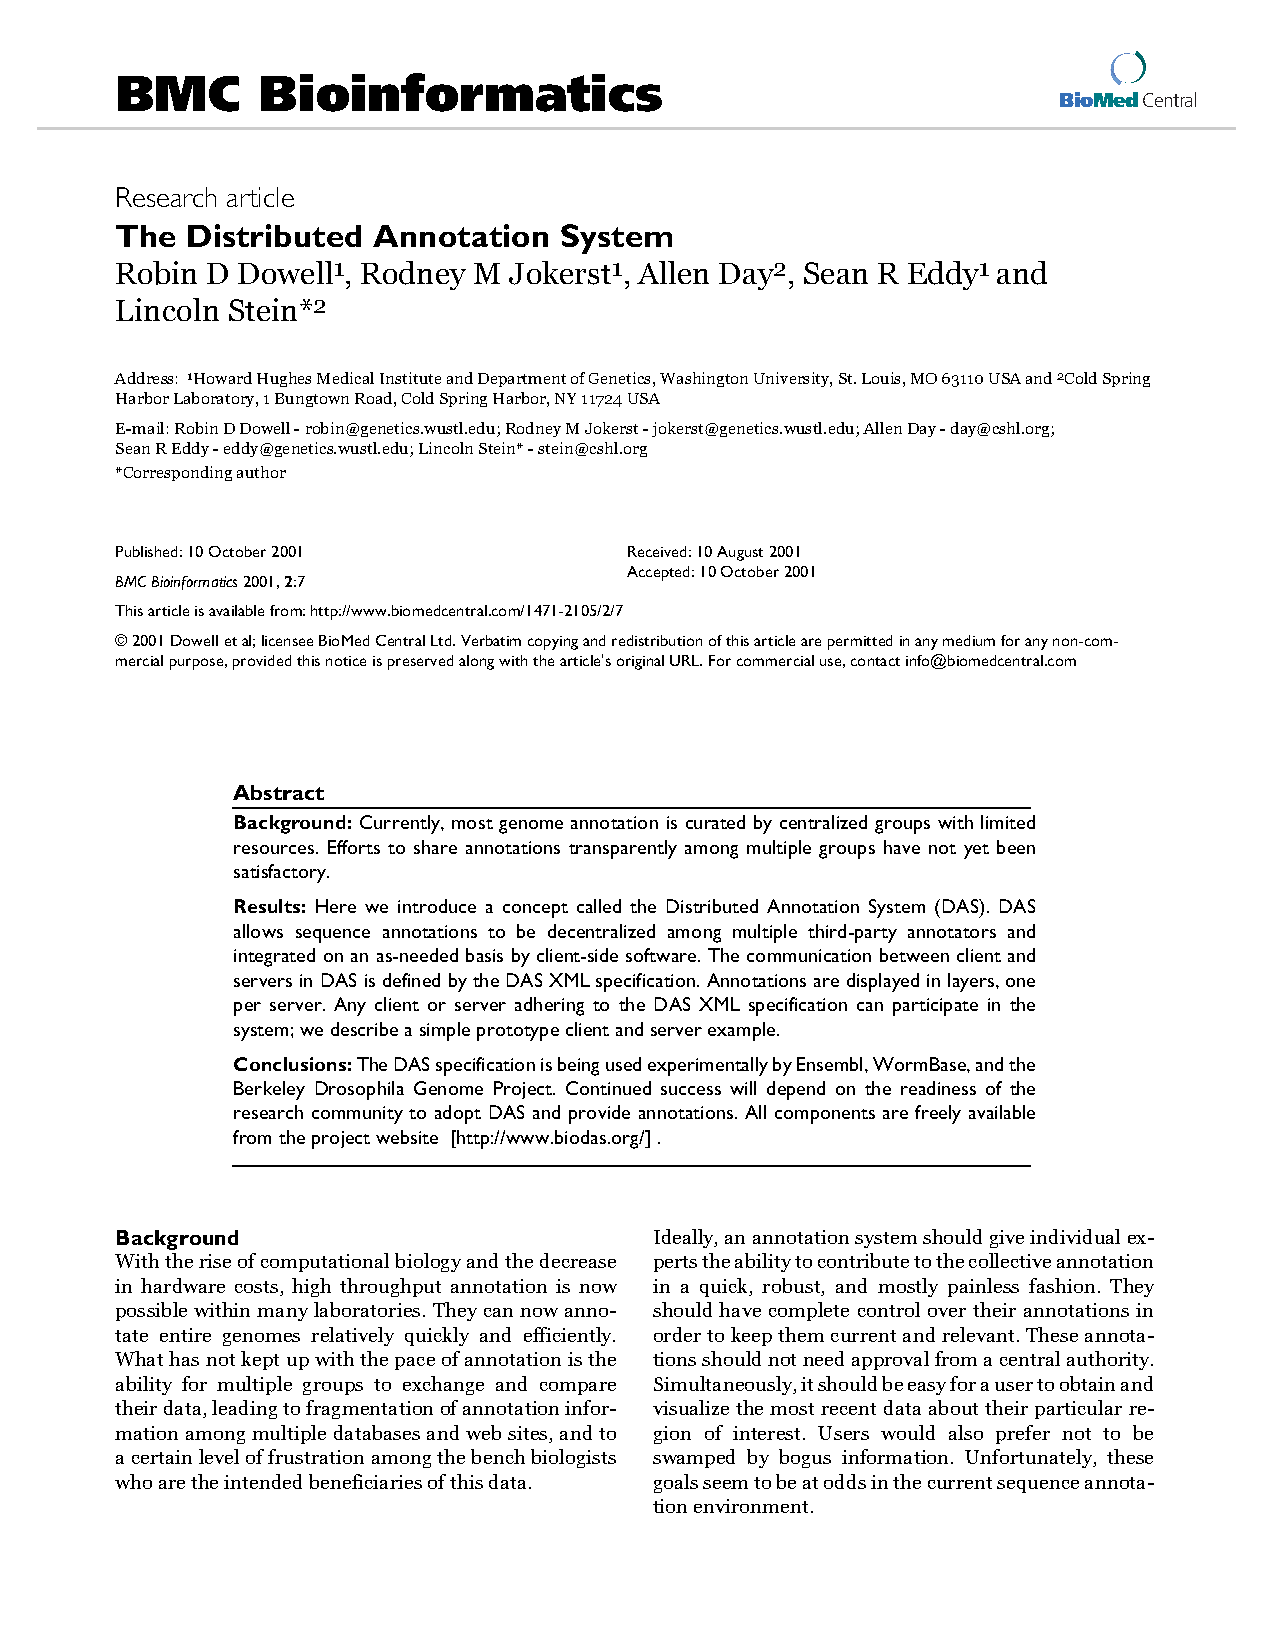
\includepdf[pages=1-7, scale=.75,
            trim=5mm 18mm 10mm 25mm,
            clip, pagecommand={}]{publications/das.pdf}

%cho paper - margins preliminary ok
\chapter{Distinct Transcription Profiles of Primary and Secondary Glioblastoma
Subgroups}
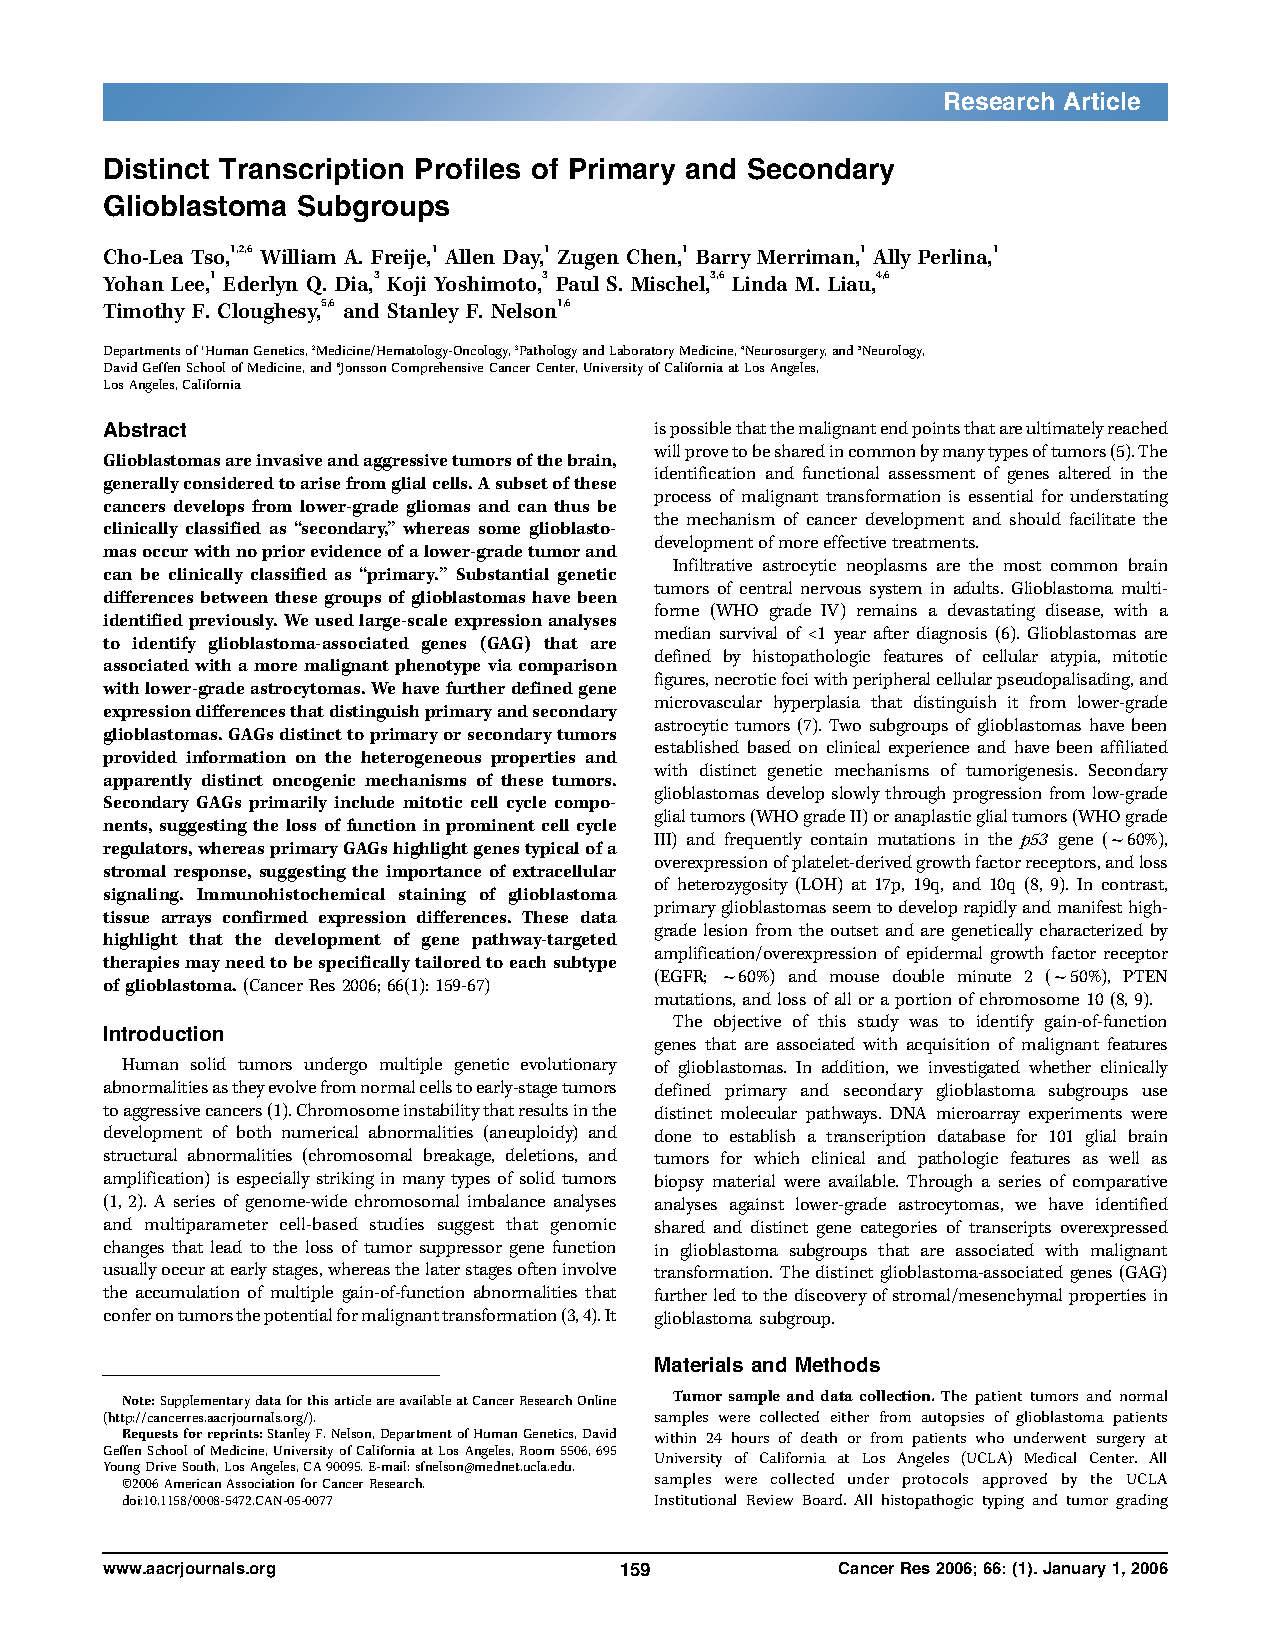
\includepdf[pages=1-9, scale=.75,
            trim=5mm 20mm 10mm 20mm,
            clip, pagecommand={}]{publications/cho.pdf}
%funari paper - magins preliminary ok
\chapter{Cartilage-selective genes identified in genome-scale analysis of
non-cartilage and cartilage gene expression.}
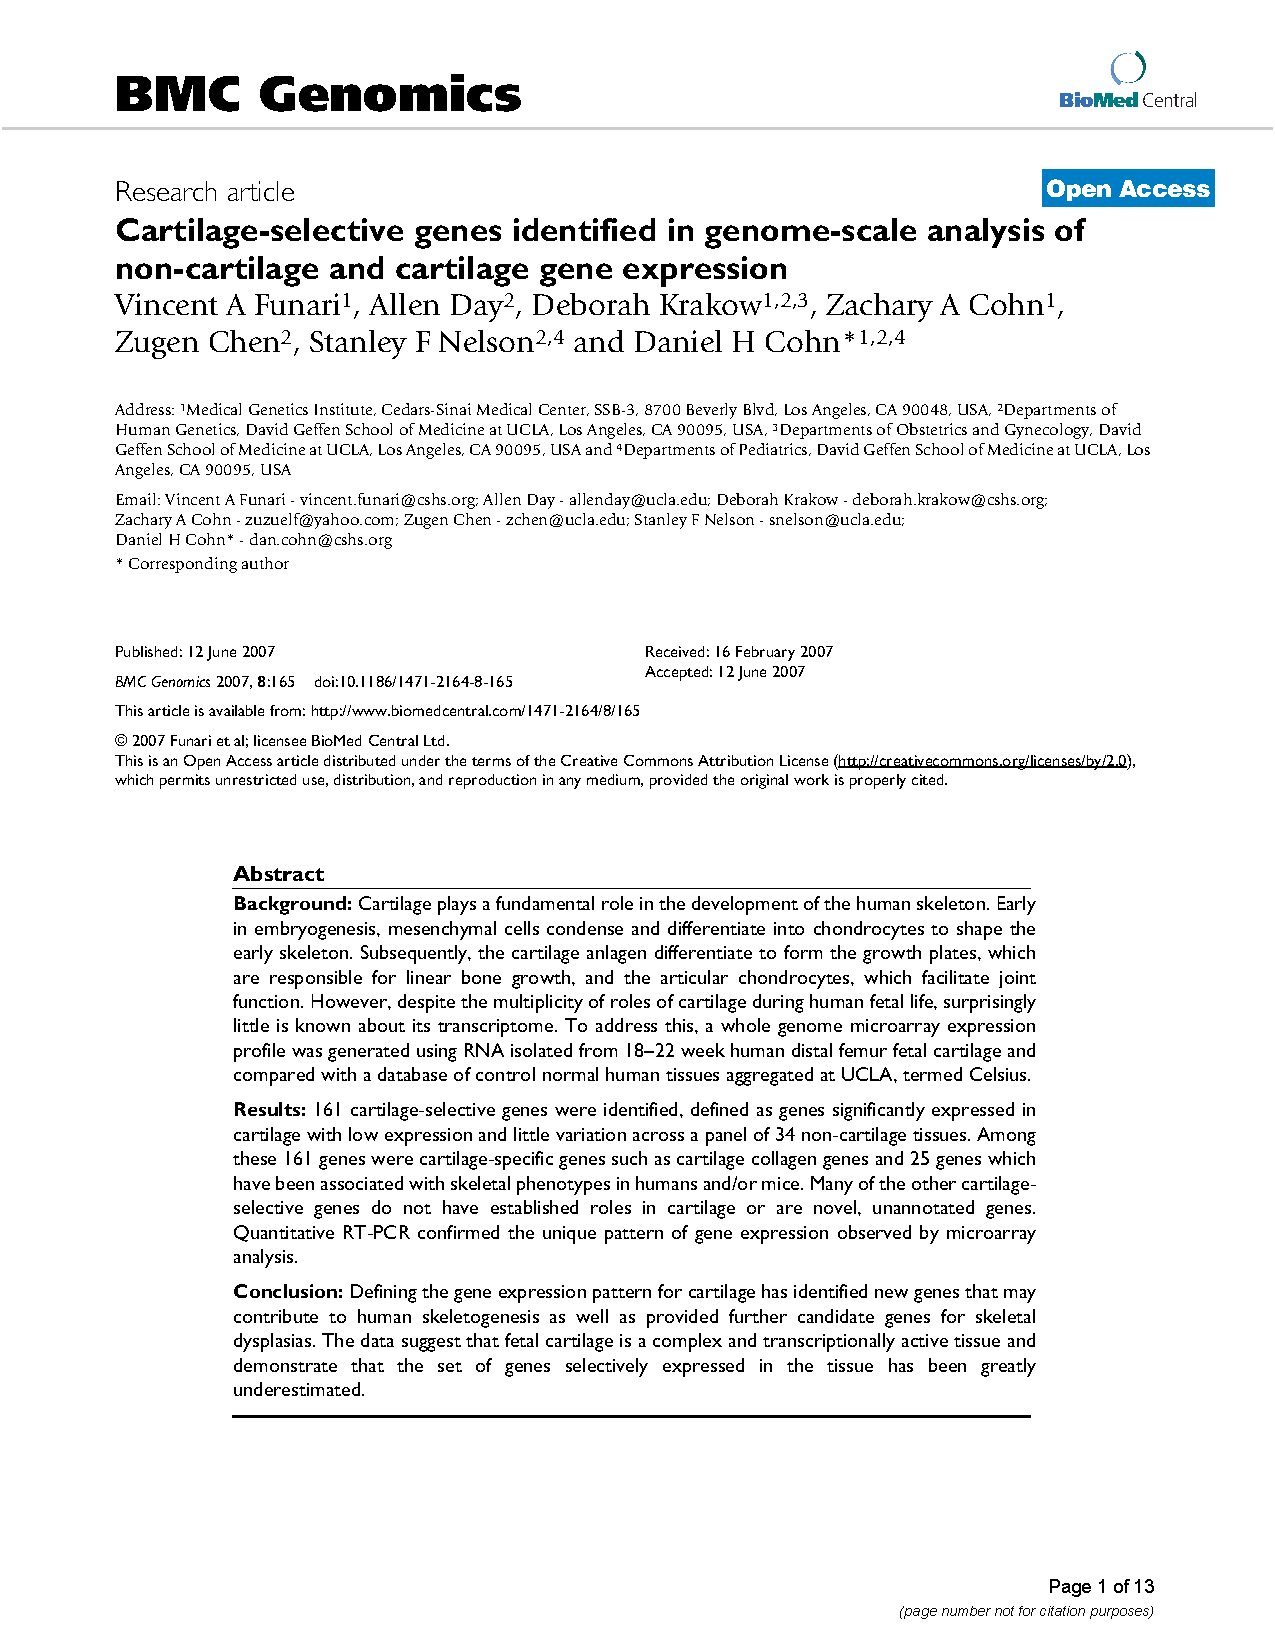
\includepdf[pages=1-4, scale=.75,
            trim=10mm 15mm 10mm 20mm,
            clip, pagecommand={}]{publications/funari.pdf}
\includepdf[pages=5-6, scale=.75,
            trim=18mm 15mm 13mm 20mm,
            clip, pagecommand={}]{publications/funari.pdf}
\includepdf[pages=7-13, scale=.75,
            trim=10mm 15mm 10mm 20mm,
            clip, pagecommand={}]{publications/funari.pdf}
\end {document}
